%%%%%Präambel%%%%%

\documentclass[12pt,a4paper]{article}%Schriftgröße, Papierformat einstellen
%\documentclass{scrbook}
\usepackage[top=30mm,bottom=30mm]{geometry}
\usepackage{lipsum}
\usepackage{csquotes}
%Pakete laden zur deutschen Rechtschreibung und für Umlaute
\usepackage[T1]{fontenc}
\usepackage[ngerman]{babel}
\usepackage[utf8]{inputenc} %für Windows, Linux
%\usepackage[applemac]{inputenc} %für Mac
%\usepackage{xcolor}
\usepackage{graphicx}
\usepackage{caption}
\usepackage[dvipsnames]{xcolor}
\usepackage{cancel}
\usepackage{titlesec}
\usepackage{cite}
\usepackage{filecontents}
\usepackage{tabularx}
\usepackage{harvard}
\usepackage{units}
\usepackage{longtable} 
\usepackage{multirow}
\usepackage{chngcntr}
\usepackage{stmaryrd}
\usepackage{array}
\usepackage{autobreak}
\usepackage{booktabs}
\usepackage{float}
\usepackage{wrapfig}
\usepackage{hhline}
\let\harvardleftorig\harvardleft
%\usepackage[round]{natbib}
%\usepackage{hyperref}
\usepackage[nottoc,numbib]{tocbibind}

%Pakete laden zu mathematischen Symbolen etc.
\usepackage{calc} 
\usepackage{amsmath,amssymb,amsthm,amsopn}
\usepackage{scrpage2}
\pagestyle{scrheadings}
\clearscrheadfoot
\automark[chapter]{section}
\ofoot{\pagemark}
\ifoot{}
\chead{\headmark}
\setfootsepline{1pt}
\setheadsepline{1pt}
%\setheadsepline[\textwidth+20pt]{0.5pt}

\DeclareMathOperator{\grad}{grad}
\DeclareMathOperator{\diverg}{div}
\DeclareMathOperator{\rot}{rot}
\DeclareMathOperator{\spur}{spur}
\DeclareMathOperator{\determ}{det}

%Inhaltsverzeichnis mit Links erstellen
\usepackage[colorlinks,
pdfpagelabels,
pdfstartview = FitH,
bookmarksopen = true,
bookmarksnumbered = true,
linkcolor = black,
plainpages = false,
hypertexnames = false,
citecolor = black] {hyperref}

% Umgebungen für Definitionen, Sätze, usw.
\newtheorem{satz}{Satz}[section]
\newtheorem{definition}[satz]{Definition}     
\newtheorem{lemma}[satz]{Lemma}	
\newtheorem{bem}{Bemerkung}[section]
% Es werden Sätze, Definitionen etc innerhalb einer Section mit
% 1.1, 1.2 etc durchnummeriert, ebenso die Gleichungen mit (1.1), (1.2) ..                  
\numberwithin{equation}{section}

\setcounter{secnumdepth}{4}
\setcounter{tocdepth}{4}

\titleformat{\paragraph}
{\normalfont\normalsize\bfseries}{\theparagraph}{1em}{}
\titlespacing*{\paragraph}
{0pt}{3.25ex plus 1ex minus .2ex}{1.5ex plus .2ex}

%neue Befehle definieren
\newcommand{\R}{\mathbb{R}} %zB \R als Abkürzung für das Symbol der reellen Zahlen
\newcommand{\N}{\mathbb{N}}
\newcommand{\Z}{\mathbb{Z}}
\newcommand{\Q}{\mathbb{Q}}
\newcommand{\C}{\mathbb{C}}
\newcommand{\diffp}{\partial}
\newcommand{\laplace}{\Delta}

\newcommand{\subsubsubsection}{\paragraph}
\newcommand\citevgl
{\def\harvardleft{(vgl.\ \global\let\harvardleft\harvardleftorig}%
 \cite
}
\newcommand\citeVgl
{\def\harvardleft{(Vgl.\ \global\let\harvardleft\harvardleftorig}%
 \cite
}

\newcommand{\tabitem}{~~\llap{\textbullet}~~}

\def\ccite#1#2{\glqq #1\grqq\cite{#2}}

\newcolumntype{L}[1]{>{\raggedleft\let\newline\\\arraybackslash\hspace{0pt}}m{#1}}
%Makros
%Makro Color
%#1 Text
\def\colBord#1{\begingroup\color{Fuchsia}{#1}\endgroup}
\def\colRed#1{\begingroup\color{Red}{#1}\endgroup}
\def\colGreen#1{\begingroup\color{LimeGreen}{#1}\endgroup}
\def\colBlue#1{\begingroup\color{NavyBlue}{#1}\endgroup}

\def\usGreen#1#2{\underset{\colGreen{#1}}{#2}}
\def\usBord#1#2{\underset{\colBord{#1}}{#2}}

\def\ubGreen#1#2{\underbrace{#2}_{\colGreen{#1}}}

\def\defF{\textbf{Def.: }}
\def\mDef#1{
\begin{definition}
  #1
\end{definition}}

\def\vecT#1{\left(\begin{array}{c} #1 \end{array}\right)}
\def\dddot{\cdot \\ \cdot \\ \cdot}
\def\vecD#1{\vecT{#1_1 \\ \dddot \\ #1_d}}
\def\vecDt#1#2{\vecT{#1 \\ \dddot \\ #2}}
\def\vecN{\mathcal{O}}
\def\vspan#1{span \lbrace #1 \rbrace}
\def\vdim#1{dim \lbrace #1 \rbrace}
\def\vker#1{ker \lbrace #1 \rbrace}
\def\vrang#1{Rang \lbrace #1 \rbrace}
\def\mzxz#1#2#3#4{\left(\begin{array}{c c} #1 & #2 \\ #3 & #4 \\ \end{array}\right)}
\def\mdxd#1#2#3{\left(\begin{array}{c c c} #1 \\ #2 \\ #3 \end{array}\right)}
\def\dfp#1#2{\frac{\partial #1}{\partial #2}}
\def\diff#1#2{\frac{\mathrm{d}#1}{\mathrm{d}#2}}

\def\epsF{\pmb{\varepsilon}}

\def\multiTwo#1#2{\multicolumn{2}{>{\hsize=\dimexpr2\hsize+2\tabcolsep+\arrayrulewidth\relax}#1}{#2}}
\def\multiThree#1#2{\multicolumn{3}{>{\hsize=\dimexpr3\hsize+4\tabcolsep+2\arrayrulewidth\relax}#1}{#2}}

\def\inR#1{\qquad ,\; #1 \in \R}
\def\inRs{\in \R}
\def\bracks#1{\left[ #1 \right]}
\def\abs#1{\left| #1 \right|}
\def\brac#1{\left( #1 \right)}

%laziness
\def\fermi{Fermi-Dirac-Verteilung}

\newcolumntype{L}[1]{>{\raggedleft\let\newline\\\arraybackslash\hspace{0pt}}m{#1}}
\newcolumntype{R}[1]{>{\raggedright\let\newline\\\arraybackslash\hspace{0pt}}m{#1}}



\def\formTab#1#2{
\begin{equation}
  \begin{tabularx}{12cm}{R{3cm} l l}
    #1 &: &$#2$
  \end{tabularx}
\end{equation}
}
\newcommand{\formTabL}[3]{
\begin{equation}
  \begin{tabularx}{12cm}{R{3cm} l l}
    #1 &: &$#2$ 
  \end{tabularx}
  \label{eq:#3}
\end{equation}}
\def\formTn{$ \\ $\;$ & $\;$ & $}
\def\formTnQ{$ \\ $\;$ & $\;$ & $\qquad}
\def\formTnQQ{$ \\ $\;$ & $\;$ & $\qquad \qquad}
\def\formTnQQQ{$ \\ $\;$ & $\;$ & $\qquad \qquad \qquad}

\renewcommand{\theequation}{\arabic{section}.\arabic{subsection}
.\arabic{equation}}
%Setzt den equation-Zaehler nach jeder Seite zurueck
\numberwithin{equation}{subsection}	


%\setlength\abovedisplayskip{0pt}

% Auf der Seite http://detexify.kirelabs.org/classify.html können Sie mathematische Symbole, Pfeile usw per Maus eingeben und bekommen den Latex-Befehl dafür angezeigt.
% detexify gibt es auch als App...

%jetzt beginnt das eigentliche Dokument
\begin{document}

\bibliographystyle{agsm}

\author{}
\title{\underline{HM2 Kurzzusammenfassung} \\ $\;$ \\ $\;$ \\ Florian Leuze}
\date{}

\maketitle % erzeugt den Kopf
\newpage
%\section{\underline{Inhalt}}
\tableofcontents

  \subsection*{Versionierung}
  \begin{tabular}{|p{2cm}|p{1cm}|p{1.5cm}|p{8.5cm}|}\hline
    Datum & Vers. & Kürzel & Änderung \\ \hline
    19.04.2018 & 0.1 & FL & Erzeugung Dokument; Erzeugung Inhaltsverzeichnis; Erzeugung Versionierung; Erzeugung 2.1 - 2.7.4 \\ \hline
    19.04.2018 & 0.2 & FL & Korrekturen 2.6.1 - 2.6.9 u. 2.7.1 - 2.7.2 Titel\\ \hline
    20.04.2018 & 0.2.1 & FL & Erzeugung 2.7.1.1 - 2.7.1.4; Korrektur Riemannsche Untersumme; Erzeugung Literaturverzeichnis \\ \hline
    23.06.2018 & 0.2.3 & FL & Neustrukturierung; Löschung HM1 Stoff; Erzeugung HM2 Stoff \\ \hline
    23.06.2018 & 0.2.4 & FL & Kleinere Korrekturen \\ \hline
    27.06.2018 & 0.2.5 & FL & Hinzugefügt: Bem. 2.8, 3.1, 3.2, 3.3, 3.8, 3.9.1 Schritt 5, 3.9.2 (Quadriken im $\R^2$; Korrekturen: 3.6.1.1 Fehler in Formel korrigiert, 3.6.1.3 Tippfehler korrigiert \\ \hline
    27.06.2018 & 0.2.6 & FL &  Bem. 3.6 korrigiert \\ \hline
    13.08.2018 & 0.3 & FL & Erzeugung Mehrd. Extremw., Satz über impl. Funkt., Extremwertaufgaben mit Nebenbe., Kurven/Bogenl., Wegintegrale \\ \hline
    13.08.2018 & 0.3.1 & FL & Kleinere Korrekturen \\ \hline
    18.08.2018 & 0.3.2 & FL & Kleinere Korrekturen \\ \hline
  \end{tabular}
\listoffigures

\newpage

\section{Allgemeines}
	\subsection{Trigonometrie}
	  \subsubsection{Winkelfunktionen}
	  \begin{align}
	    sin(\alpha) = \frac{Gegenkathete}{Hypothenuse}\\
	    cos(\alpha) = \frac{Ankathete}{Hypothenuse}\\
	    tan(\alpha) = \frac{Gegenkathete}{Ankathete} \label{eq:trigo_Winkelf}
	  \end{align}
	  
	  \subsubsubsection{Wichtige Werte}
	  \renewcommand{\arraystretch}{1.5}
	  \begin{tabular}{|p{3.2cm}|p{1.8cm}|p{1.8cm}|p{1.8cm}|p{1.8cm}|p{1.8cm}|}\hline
	  $\alpha$ in Gradmaß & $0^{\circ}$ & $30^{\circ}$ & $45^{\circ}$ & $60^{\circ}$ & $90^{\circ}$ \\ \hline
	  $\alpha$ in Bogenmaß & $0$ & $\frac{\Pi}{6}$ & $\frac{\pi}{4}$ & $\frac{\pi}{3}$ & $\frac{\pi}{2}$ \\ \hline
	  $sin\alpha$ & $\frac{1}{2}\sqrt{0}$ & $\frac{1}{2}\sqrt{1}$ & $\frac{1}{2} \sqrt{2}$ & $\frac{1}{2}\sqrt{3}$ & $1$ \\ \hline
	  $cos\alpha$ & $1$ & $\frac{1}{2}\sqrt{3}$ & $\frac{1}{2}\sqrt{2}$ & $\frac{1}{2}\sqrt{1}$ & $\frac{1}{2}\sqrt{0}$ \\ \hline
	  $tan\alpha$ & $0$ & $\frac{1}{3}\sqrt{3}$ & $1$ & $\sqrt{3}$ & n.d. \\ \hline
	  \end{tabular}
	  \renewcommand{\arraystretch}{1}
	  
	  \subsubsection{Sinussatz}
	  \begin{equation}
	    \frac{a}{sin\alpha} = \frac{b}{sin\beta} = \frac{c}{sin\gamma} = 2r = \frac{abc}{2F} \label{eq:allg_sinussatz}  
	  \end{equation}
	  
	  \subsubsection{Cosinussatz}
	  \begin{align}   
	    a^2 = b^2 + c^2 - 2bc cos\alpha\\
	    b^2 = c^2 + a^2 - 2ca cos\beta\\
	    c^2 = a^2 + b^2 - 2ab cos\gamma \label{eq:trigo_cosinussatz}
	  \end{align}
	  
	  \subsubsection{Tangenssatz}
	  \begin{align}
	    \frac{b + c}{b - c} = \frac{tan\left(\frac{\beta + \gamma}{2}\right)}{tan\left(\frac{\beta - \gamma}{2}\right)} 
	    = \frac{cot\left(\frac{\alpha}{2} \right)}{tan\left(\frac{\beta - \gamma}{2}\right)}
	  \end{align}
	  Analog für $\frac{a + b}{a - b}$ und $\frac{a + c}{a - c}$.\label{eq:trigo_tangenssatz}
	  
	  \subsubsection{Umwandlung}
	  \begin{align}
	    \cos t \sin t = \frac{1}{2} \left(e^{it}+e^{-it}\right) \frac{1}{2i}\left(e^{i2t} - e^{-i2t}\right) &= \frac{1}{2} \frac{1}{2i}\left( e^{i2t}-e^{-i2t}\right) = \frac{1}{2}\sin 2t\\
	    tan\alpha &= \frac{sin\alpha}{cos\alpha}\\
	    sin^2(\alpha) + cos^2(\alpha) &= 1\\
	    1 + tan^2(\alpha) = \frac{1}{cos^2(\alpha)} &= sec^2(\alpha)\\
	    1 + cot^2(\alpha) = \frac{1}{sin^2(\alpha)} &= csc^2(\alpha)\label{eq:trigo_umwandlung}
	  \end{align}
	  
	  \subsubsection{Additionstheoreme}
	  \begin{align}
	    sin(x \pm y) &= sin(x) cos(y) \pm cos(x) sin(y)\\
	    cos(x \pm y) &= cos(x) cos(y) \mp sin(x) sin(y)\\\\
	    tan(x \pm y) &= \frac{tan(x) \pm tan(y)}{1 \mp tan(x) tan(y)} = \frac{sin(x \pm y)}{cos(x \pm y)}\\
	    cot(x \pm y) &= \frac{cot(x) cot(y) \mp 1}{cot(y) \pm cot(x)} = \frac{cos(x \pm y)}{sin(x \pm y)}\\\\
	    sin(x + y) \cdot sin(x - y) &= cos^2(y) - cos^2(x) = sin^2(x) - sin^2(y)\\
	    cos(x + y) \cdot cos(x - y) &= cos^2(y) - sin^2(x) = cos^2(x) - sin^2(y)\label{eq:trigo_addtheo}
	  \end{align}
	  
	  \subsubsection{Folgerungen aus den Additionstheoremen}
	  \begin{align}
	  cos^2(\frac{x}{2}) + sin^2(\frac{x}{2}) &\;\;= cos(\frac{x}{2}) cos(\frac{x}{2}) + sin(\frac{x}{2}) sin(\frac{x}{2})\\ 
	  &\overset{\eqref{eq:trigo_addtheo}}{=} cos(\frac{x}{2}-\frac{x}{2}) = cos(0) = 1\\
	  \\
	  2sin(\frac{x}{2})cos(\frac{x}{2}) &\;\;= sin(\frac{x}{2})cos(\frac{x}{2}) + sin(\frac{x}{2})cos(\frac{x}{2})\\
	  &\overset{\eqref{eq:trigo_addtheo}}{=} sin(\frac{x}{2}+ \frac{x}{2}) = sin(x)\\
	  \\
	  sin(2x) = sin(x+x) &\overset{\eqref{eq:trigo_addtheo}}{=} sin(x)cos(x) + sin(x)cos(x) \\
	  &\;\;=2sin(x)cos(x) \label{eq:trigo:addtheo_folg}
	  \end{align}
\newpage

\section{Integralberechnung}
\subsection{Unbestimmtes Integral}
\begin{equation}
\int f(x) dx = F(x) + C = [F(x)]\qquad, C\in\R \label{eq:def_noBorder}
\end{equation}

\subsection{Bestimmtes Integral}
\begin{equation}
\int_a^b f(x) dx = F(b) - F(a) \label{eq:def_border}
\end{equation}

\subsection{Partielle Integration}
Entspricht der "Produktregel" der Differentialrechnung.
\begin{equation}
\int_{\colBord{a}}^{\colBord{b}} f'(x) g(x) dx = f(x) g(x) \colBord{\Big|_a^b} - \int_{\colBord{a}}^{\colBord{b}} f(x) g'(x) dx \label{eq:rule_partInt}
\end{equation}
Bietet sich zum Beispiel bei Produkten aus x-Potenz mit e-Funktionen, log, sin oder cos an.

\subsection{Integration durch Substitution}
Entspricht der "Kettenregel" der Differentialrechnung.
\begin{equation}
\int_{\colBord{a}}^{\colBord{b}} f(g(x))g'(x) dx = \int_{\colBord{g(a)}}^{\colBord{g(b)}} f(y) dy \qquad (setze \quad y = g(x) \label{eq:rule_subs}
\end{equation}

\subsubsection{Spezialfall}
\begin{equation}
\int \frac{f'(x)}{f(x)} dx = ln(|f(x)|) + C \qquad ,C\in\R \label{eq:rule_spec}
\end{equation}

\subsection{Gerade/Ungerade Funktionen}
\begin{align}
\int_{-a}^a f(x) = 
\begin{cases}
2 \int_0^a f(x) dx &,\; f\; gerade\\
0 &,\; f\; ungerade\\
\end{cases} \label{eq:evenodd}
\end{align}
\begin{align*}
\text{f gerade, falls }f(-x) &= f(x) \qquad &(z.B.: cos(x), x^2)\\
\text{f ungerade, falls }f(-x) &= -f(x) \qquad &(z.B.: sin(x), x^3)\\
\end{align*}

\subsection{Allgemeines zur Integration}
\subsubsection{Riemann Integrierbarkeit}
$f:[a,b] \rightarrow \R$ stetig bzw. monoton \newline
$\Rightarrow$ f ist R-integrierbar.

\subsubsubsection{Riemannsches Unterintegral}
\begin{equation}
\int_{a}^{\bar{b}} f(x) dx = \sup\{U_f(Z): \; \text{Z Zerlegung von }[a,b]\}
\end{equation}


\subsubsubsection{Riemannsches Oberintegral}
\begin{equation}
\int_{\bar{a}}^{b} f(x) dx = \inf\{O_f(Z): \; \text{Z Zerlegung von }[a,b]\}
\end{equation}

$\rightarrow \text{f heißt Riemann-integrierbar über }[a,b]$, falls
\begin{equation}
\int_{\bar{a}}^{b} f(x) dx = \int_a^{\bar{b}} f(x) dx
\end{equation}
\newline
In diesem Fall heißt der Wert das Riemannn-Integral und wird mit $\int_a^b f(x)dx$ bezeichnet.

\subsubsubsection{Riemannsche Untersumme}
\begin{equation}
  U_f(Z) = \sum_{j = 0}^{n-1} \inf\limits_{\xi \in [x_j, X_{j+1}]} f(\xi) \cdot (x_{j+1} -x_j)
\end{equation}
\subsubsubsection{Riemannsche Obersumme}
\begin{equation}
  O_f(Z) = \sum_{j = 0}^{n-1} \sup\limits_{\xi \in [x_j, X_{j+1}]} f(\xi) \cdot (x_{j+1} -x_j)
\end{equation}

\subsubsubsection{Eigenschaften}
\begin{description}
\item[a)]
Falls $a<b$ setzen wir:
\begin{align}
\int_b^a f(x) dx &= -\int_a^bf(x)dx \nonumber \\
\int_a^a f(x) dx &= 0
\end{align}
\item[b)]
f, g seien R-integrierbar, $\lambda , \mu \in \R \rightarrow \lambda f + \mu g$ ist R-integrierbar (Vektorraumeigenschaft).
\begin{equation}
\int_a^b \lambda f + \mu g)(x)dx = \lambda \int_a^b f(x) dx + \mu \int_a^b g(x) dx
\end{equation}
\item[c)]
$a<C<b$, f ist R-integrierbar.
\begin{equation}
\int_a^b f(x) dx = \int_a^C f(x) dx + \int_C^b f(x) dx
\end{equation}
\item[d)]
\begin{align}
f(x) \ge 0 &\Rightarrow \int_a^b f(x) dx \ge 0 \nonumber \\
f(x) \ge g(x) &\Rightarrow \int_a^b f(x) dx \ge \int_a^b g(x)dx
\end{align}
\item[e)]
\begin{equation}
\text{Sind $f$ und $g$ R-integrierbar ist auch $f*g$ R-integrierbar.}
\end{equation}
\item[f)]
\begin{align}
g(x) \ge C > 0 \Rightarrow \frac{f}{g} \text{ ist R-integrierbar.}
\end{align}
\item[g)]
\begin{equation}
\text{Ist $f$ R-integrierbar dann ist auch } |f| \text{ R-integrierbar.}
\end{equation} 
\item[h)]
\begin{equation}
(b-a) \inf_{x\in[a,b]}{f(x)} \le \int_a^b f(x) dx \le (b-a) \sup_{x\in [a,b]}{f(x)}
\end{equation}
\end{description}

\subsubsubsection{Kriterien zur Riemann-Integrierbarkeit}

\begin{description}
\item[a)]
$f$ monoton $\Rightarrow f$ R-integrierbar.
\item[b)]
$f$ stetig $\Rightarrow f$ R-integrierbar
\begin{satz}
\glqq Jede stetige Funktion $f:k \rightarrow \R$ auf einer kompakten Menge k, d.h. für $k<\R^d$ abgeschlossen und beschränkt, ist dort gleichmäßig stetig und damit R-integrierbar.\grqq \cite{HM12}
Beispiel für k: $k:[a,b]$
\end{satz}
\item[c)]
\begin{satz}
Kriterium: Jede Funktion deren Unstetigkeitsstellen eine Nullmenge bilden (z.B. abzählbare Mengen) sind R-integrierbar.
\glqq Satz: Eine Funktion $f:[a,b]\rightarrow \R$ ist genau dann R-integrierbar, wenn $f$ beschränkt ist und die Menge der Unstetigkeitsstellen eine Nullmenge ist. 
\grqq \cite{HM12}
\end{satz}
Die Konsequenz daraus lautet, dass jede stetige Funktion mit endlich vielen Sprungstellen R-integrierbar ist. \citeVgl{HM12}
\item[d)]
\begin{satz}
\glqq Sei $f:[a,b] \rightarrow \R$ beschränkt. Dann ist $f$ R-integrierbar genau dann, wenn es zu jedem $\varepsilon > 0$ eine Partition $Z$ gibt, 
so dass
$O_f(Z)  U_f(Z) < \varepsilon$. \grqq \cite{HM12}
\end{satz}
Anmerkung: \glqq In der Mengenlehre ist eine Partition (auch Zerlegung oder Klasseneinteilung) einer Menge M eine Menge P, deren Elemente nichtleere Teilmengen von M sind, sodass jedes Element von M in genau einem Element von P enthalten ist. Anders gesagt: Eine Partition einer Menge ist eine Zerlegung dieser Menge in nichtleere paarweise disjunkte Teilmengen.\grqq  \cite{wiki}

\end{description}

\subsubsection{MWS der Integralrechnung}
$f:[a,b]\rightarrow\R$ stetig, dann $\exists \; \xi \in[a,b]$ mit $\int_a^b f(x)dx = f(\xi)(b-a)$.

\subsubsection{Hauptsatz der Differential- und Integralrechnung}
$f:[a,b]\rightarrow\R$ stetig, dann ist $F(x) = \int_a^x f(t)dt$ diffbar und $F'(x) = f(x)$.

\subsubsubsection{Folgerungen}
\begin{satz}
Ist $f$ ungerade, so ist $f''$ gerade, und alle Stammfunktionen vonm $f$ sind gerade.\citevgl{HM2Vortragsubung}
\end{satz}
\begin{satz}
Ist $f$ gerade, so ist $f'$ ungerade, und $f$ besitzt eine ungerade Stammfunktion.\citevgl{HM2Vortragsubung}
\end{satz}

\subsection{Partialbruchzerlegung}
	\begin{equation}
	  R(x) = \frac{p(x)}{q(x)}, \qquad p,q\text{ Polynome}
	\end{equation}
	Vorgehensweise:
	\begin{description}
	  \item{\textbf{1)}} Zähler und Nennergrad untersuchen\newline
	  ist $grad(p) > grad(q)$, also Zählergrad > Nennergrad umformen in  \newline$R(x) = p_1(x) + \frac{p_2(x)}{q(x)}$ $\Rightarrow$ Polynomdivision.
	  \item{\textbf{2)}} Nullstellen und faktorisieren
	    \begin{itemize}
	      \item Nullstellen des Nenners bestimmen
	      \item Nenner Faktorisieren in $p1, p2, ...$
	    \end{itemize}
	  \item{\textbf{3)}} Ansatz
	    \begin{itemize}
	      \item Ansatz für Partialbruchzerlegung $R(x) = \frac{A}{p1} + \frac{B}{p2} + ...$
	      \item Bestimmung von A, B, C, ...
	    \end{itemize}
	\end{description}
  Bei quadratischen oder höhergradigen Nullstellen lautet der Ansatz:
  \begin{equation}
    NST = x^n \Rightarrow R(x) = \frac{A}{x} + \frac{B}{x^2} + ... + \frac{N}{x^n}
  \end{equation}
  Bei komplexen Nullstellen muss der Ansatz angepasst werden.
  \begin{align}
    &NST: 2, -2, 2i, -2i \nonumber \\
    &Ansatz: R(x) = \frac{A}{x-2} + \frac{B}{x+2} + \frac{Cx + D}{x^2+4}
  \end{align}
  Es werden also die komplexen Nullstellen ausmultipliziert und so reell dargestellt.
  
\subsection{Uneigentliche Integrale}
  \begin{satz}
    Sei $f:[a, \infty] := I \rightarrow \R$ lokal integrierbar. Konvergiert $\int_a^\infty f(x) dx$ absolut. d.h. ist $\int_a^\infty |f(x)| dx$ konvergent, so konvergiert auch $\int_a^\infty f(x) dx$.
  \end{satz}
  \begin{satz}
    Majorantenkriterium: Gilt für alle $x\in I$, dass $|f(x)| \leq g(x)$, und ist $\int_a^\infty g(x) dx$ konvergent, so ist $\int_a^\infty dx$ (im Script vom Prof ist hier die untere Grenze 0, ich denke es sollte aber a sein) absolut konvergent.    
  \end{satz}
  \begin{satz}
    Minorantenkriterium: Gilt für alle $x\in I$, dass $0 \leq g(x) \leq f(x)$ und divergiert $\int_a^\infty g(x) dx$, so divergiert auch $\int_a^\infty dx$.
  \end{satz}
  \begin{bem}
    Abschätzungen mit negativen Minoranten sind falsch da mit einer negativen Minorante alles nach unten abgeschätzt werden kann.
  \end{bem}
  \subsubsection{Typen uneigentlicher Integrale}
  \begin{align}
    \textbf{\colGreen{Singularität:} }\int_{\colGreen{0}}^1 \frac{1}{\sqrt{\colGreen{x}}} dx \nonumber \\
    \textbf{\colGreen{Unbeschränktes Gebiet:} }\int_1^{\colGreen{\infty}} e^{-x} dx \nonumber \\
  \end{align}
  \begin{definition}
    Eine Singularität ist die Stelle, an der die Funktion divergieren würde oder undefiniert wäre.
  \end{definition}
  \textbf{Methode:} Ersetzen der kritischen Stelle durch $z$ und setzen eines Grenzüberganges, z.B.:
  \begin{align*}
    \lim\limits_{z\rightarrow0} \int_z^1 \frac{1}{\sqrt{x}} dx, \quad \lim\limits_{z\rightarrow \infty} \int_1^z e^{-x} dx
  \end{align*}
  \textbf{Vergleichsintegrale}
  \begin{align}
    \int_1^\infty \frac{1}{x^\alpha} dx = 
    \begin{cases}
      \text{konvergiert}\quad , \alpha > 1 \\
      \text{divergiert}\quad , \alpha \leq 1
    \end{cases} \nonumber\\
    \int_0^1 \frac{1}{x^\alpha} dx = 
    \begin{cases}
      \text{divergiert}\quad , \alpha \geq 1 \\
      \text{konvergiert}\quad , \alpha < 1
    \end{cases} \nonumber\\    
  \end{align}

\subsection{Wichtige Integrale}
\begin{equation}
  \int \frac{1}{1+y^2} dx = arctan(y)
\end{equation}
\begin{equation}
  \int x^n dx = \frac{x^{n+1}}{n+1}, \qquad n \neq -1
\end{equation}
\begin{equation}
  \int \frac{1}{cos^2(x)} dx = tan(x)
\end{equation}
\begin{equation}
  \int \frac{1}{sin^2(x)} dx = cot(x)
\end{equation}
\begin{equation}
  \int a^x dx = \frac{a^x}{ln(a)}
\end{equation}
\begin{equation}
  \int \frac{1}{x} dx = ln|x|
\end{equation}
\begin{equation}
  \int \frac{1}{cosh^2(x)} dx = tanh(x)
\end{equation}
\begin{equation}
  \int \frac{1}{sinh^2(x)} dx = -coth(x)
\end{equation}
\begin{equation}
  \int ln(x) dx = x ln(x) -x
\end{equation}
\begin{equation}
  \int \frac{1}{x-x_1} dx = ln|x-x_1|
\end{equation}
\begin{equation}
  \int \frac{1}{/x-x_1)^k} dx = \frac{1}{-k+1}(x-x_1)^{-k+1}, \quad k>1
\end{equation}
\begin{equation}
  \int \frac{1}{(x-a)^2+b^2}dx = \frac{1}{b^2} \int \frac{1}{\left(\frac{x-a}{b}\right)^2 +1} dx = \frac{1}{b} arctan\left(\frac{x-a}{b}\right)
\end{equation}

\subsection{Separierbare DGL}
  \subsubsection{Wiederholung klassische DGL}
  Bisher: lineare DGl mit konstanten Koeffizienten. \newline
  z.B.: $y''(t) - 5y'(t) + 4y(t) = e^{\colGreen{2}t} \qquad ,\; y(0) = 1,\; y'(0) = 1$ \newline
  \begin{tabularx}{14.7cm}{l l}
	  Homogene DGL: & $y(t) = e^{\lambda t} \Rightarrow p(\lambda) = \lambda^2 - 5 \lambda +4 = 0$ \\
	  $\;$ & $\Rightarrow \lambda_1 = 1, \; \lambda_2 = 4$ \\
	  $\;$ & $\Rightarrow yh(t) = C_1 e^t + C_2 e^{4t} \qquad ,\;C_1,\;C_2 \in \R$\\
	  $\;$ & $\;$ \\
	  Inhomogenes DGL: & $\ubGreen{\text{da 2 keine NST}}{yp(t) = re^{2t}}$\\
  \end{tabularx}  
  \begin{align*}
    &\Rightarrow yp'(t) = 2re^{2t},\; yp''(t) = 4re^{2t} \\
    &\overset{DGL}{=} 4re^{2t} - 10re^{2t} + 4re^{2t} \overset{!}{=} e^{2t} \Rightarrow -2re^{2t} = e^{2t}\\
    &\Rightarrow r = -\frac{1}{2}
  \end{align*} 
  \begin{tabularx}{14.7cm}{l l}
	  Allgemeine Lösung: & $y(t) = yh(t) + yp(t) = C_1 e^t + C_2 e^{4t} - \frac{1}{2} e^{2t}$
  \end{tabularx}
  
  \subsubsection{Lösen von DGL mit Koeffizienten die von t abhängig sind}
  z.B. $ y'(t) - ty(t) = t \qquad ,\; y(0) = 1$\newline
  \newline
  Spezielle Form: 
  \begin{equation}
    y'(t) = f(t) g(y(t)) \qquad,\; y(t_0) = y_0
  \end{equation}     
  \begin{align*}
    \Rightarrow y'(t) = t+ty(t) = \ubGreen{f(t)}{t} \ubGreen{(1+y(t))}{g(y(t))}
  \end{align*}
  Lösung: Trennung der Veränderlichen:
  \begin{align}
  \frac{y'}{g(y)} = f(t) \overset{\colGreen{y' = \frac{dy}{dt}}}{\Rightarrow} \colGreen{\int} \frac{1}{g(y)} dy = \colGreen{\int} f(t)dt +C \quad ,\;C\in\R
  \end{align}
  $C$ erhält man aus der Anfangsbedingung $y(t_0) = y_0$.
  \newpage
	
\section{Lineare Algebra}
  \subsection{Definitionen}
  \subsubsection{Linearkombinationen}
  $V$ sei ein Vektorraum (im Folgenden VR), $v_1,\;...,\;v_m \in V\quad ,\;\lambda  _i \in \R$.
  \begin{equation}
		  \begin{tabularx}{14.7cm}{l l l}
				(\textbf{1}) & $\sum\limits_{i = 1}^m \lambda_i v_i$ & \colBlue{Linearkombinationen der $v_i$.}\\
		  \end{tabularx}
		  \label{def:linA_lineark}
    \end{equation}
    \subsubsection{Spann und Erzeugendensystem}
    \begin{equation}
		  \begin{tabularx}{14.7cm}{l l l}
				(\textbf{2}) & $span(v_1,\;...,\;v_m) = \left\lbrace \sum\limits_{i = 1}^m \lambda_i v_i \quad ,\; \lambda_i,\; \in \R,\;  v_i  \in V \right\rbrace$ & \colBlue{Spann der
				 $v_i$.}\\
				 $\;$ & Gilt $span(v_1,\;...,\;v_m) = V \Rightarrow \lbrace v_1,\;...,\;v_m \rbrace$ &ist ein Erzeugendensystem.\\
		  \end{tabularx}
		  \label{def:linA_span}
    \end{equation}
    \begin{bem}
      Es gilt:
      \begin{equation}
        dim = span \Rightarrow EZS
      \end{equation}
    \end{bem}
    \subsubsection{Lineare Unabhängigkeit}
    \begin{equation}
		  \begin{tabularx}{14.7cm}{l l l}
				(\textbf{3}) & \multiTwo{l}{$v_1,\;...,\;v_m$ linear unabhänig, falls}\\ 
				$\;$ & \multiTwo{l}{$\sum\limits_{i = 1}^m \lambda_i v_i = \vec{0} \Rightarrow \lambda_1 = \lambda_2 = ... = \lambda_m = 0$}\\
				$\;$ & \multiTwo{l}{$0$ darf die einzige Lösung sein, sonst linear abhängig.}\\
		  \end{tabularx}
		  \label{def:linA_linearabh}
    \end{equation}
    \begin{bem}
      Es gilt:
      \begin{equation}
        detA \neq 0 \Rightarrow \text{linear unabhängig}
      \end{equation}
    \end{bem}
    \subsubsection{Basis}
    \begin{equation}
		  \begin{tabularx}{14.7cm}{l l l}
				(\textbf{4}) & \multiTwo{l}{$B = \lbrace b_1,\;...,\;b_n \rbrace \subset V$ ist Basis von $V$, falls}\\
				$\;$ & \colGreen{(B1)} & $b_i$ linear unabhängig, $i = 1,\; ...,\; n$\\
				$\;$ & \colGreen{(B2)} & $B$ ist ein Erzeugendensystem.\\
		  \end{tabularx}
		  \label{def:linA_basis}
    \end{equation}	
    
    Es gilt:
    \begin{equation}
      \begin{tabularx}{14.7cm}{l l l}
      (\textbf{1}) & $dimV = |b|$ & \colBlue{(Mächtigkeit von $B$)}\\
      (\textbf{2}) & $dimV = n$ & \colBlue{($\Rightarrow n+1$ Vektoren sind linear abhängig)}\\
      (\textbf{3}) & \multiTwo{l}{$\forall v \in V: v = \sum\limits_{i = 1}^n \lambda_i b_i$ eindeutig darstellbar.}\\
      $\;$ & $\Rightarrow B^v = (\lambda_1,\;...,\; \lambda_n)^T$ & \colBlue{(Koordinaten von $v$ bezüglich $B$)}\\
      \end{tabularx}
      \label{def:linA_allg}
    \end{equation}

  \subsubsection{Kanonische Basis}
  \begin{equation}
    e_1 = \vecT{1\\0\\ \dddot \\ 0,} \quad e_2 = \vecT{0\\1\\ \dddot \\ 0}, \quad ..., \quad e_d = \vecT{0\\ \dddot \\0 \\1}
  \end{equation}
	\subsection{Vektorräume}
		\subsubsection{Definitionen}
		\subsubsubsection{$\R^d$}
		\begin{equation}
			\R^d: v = \vecT{v_1\\v_2\\ \dddot \\v_d},\; w = \vecT{w_1\\w_2\\ \dddot \\ w_d}
		\end{equation}	
		\subsubsubsection{Vektoraddition}
		\begin{equation}
			v + w = \vecD{v} + \vecD{w} = \vecT{v_1 + w_1 \\ \dddot \\ v_d + w_d}
		\end{equation}
		\subsubsubsection{Skalare Multiplikation}
		\begin{align}
			\alpha \in \R, \; v \in \R^d \nonumber \\
			\alpha \cdot v = \vecD{\alpha\cdot v}
		\end{align}
		\subsubsubsection{Nullvektor}
		\begin{equation}
		  \mathcal{O} = \vecT{0 \\ \dddot \\ 0}
    \end{equation}		
    
    \subsubsection{Struktur}
    Für $v,\;w,\;z \in \R^d$ gelten die folgenden Eigenschaften:
    \begin{equation}
		  \begin{tabularx}{14.7cm}{l l l}
				(\textbf{V1}) & $v + w = w + v$ &\\
				(\textbf{V2}) & $v+(w+z) = (v+w)+z$ &\\
				(\textbf{V3}) & $v + 0 = 0 + v = v$ & \colBlue{(0 ist das neutrale Element)}\\
				(\textbf{V4}) & $v+(-v) = (-v)+v = 0$ & \colBlue{(-v ist das inverse Element)}\\
		  \end{tabularx}
		  \label{ax:vektorraumeig_v}
    \end{equation}	
    \newline
    Für $\alpha\; \beta \in \R,\; v,\;w \in \R^d$ gilt:
    \begin{equation}
		  \begin{tabularx}{14.7cm}{l l l}
				(\textbf{S1}) & $1 \cdot v = v$ & $\qquad\colBlue{(1\in \R)}$\\
				(\textbf{S2}) & $\alpha (\beta v) = (\alpha \beta)v$ &\\
				(\textbf{S3}) & $(\alpha + \beta) v = \alpha \cdot v + \beta \cdot v$ &\\
				(\textbf{S4}) & $\alpha(v + w) = \alpha \cdot v + \alpha \cdot w$ &\\
		  \end{tabularx}
		  \label{ax:vektorraumeig_s}
    \end{equation}		 
    $(V1) - (V4)$ und $(S1) - (S4)$ gelten auch für Funktionen.
    \begin{definition}
    Ist $V$ eine Menge für deren Elemente eine Addition und eine skalare Multiplikation erklärt ist, so heißt sie Vektorraum, falls die Eigenschaften 
    $(V1)$ - $  (V4)$ und $(S1)$ - $(S4)$ erfüllt sind, wobei jetzt $v,\;w,\;z\in V$.
    Je nach Skalarkörper, also $\R$ oder $\C$ sprechen wir von einem reellen oder komplexen Vektorraum. Teilmengen von Vektorräumen, die ebenfalls Vektorräume
    sind, heißen Untervektorräume. \cite{HM12}
    \end{definition}

	  \subsubsection{Untervektorraum}
	  $V$ sei ein Vektorraum und es gelte $U \subset V$.
	  \begin{definition}
	  Eigenschaften $(V1)$ - $(V4)$, $(S1)$ - $(S4)$ sind als Teilmenge von V erfüllt, aber mit $u,\;v \in U$ und $\alpha \in \R$ muss auch $u + v \in U$
	  , $\alpha  u \in U$ gelten (Abgeschlossenheit bezüglich Vektoraddition und skalarer Multiplikation). \cite{HM12}
	  \end{definition}
	  \subsubsubsection{Untervektorraumkriterien}
	  \begin{equation}
			  \begin{tabularx}{14.7cm}{l l l}
					(\textbf{UV0}) & $0 \in U$ &\\
					(\textbf{UV1}) & $u,\;v \in U \Rightarrow u + v \in U$ &\\
					(\textbf{UV2}) & $u \in U,\; \lambda \in \R \Rightarrow \lambda u \in U$ &\\
			  \end{tabularx}
			  \label{ax:vektorraumeig_uv}
	   \end{equation}
	   \newline
	   Es gilt: $U_1,\; U_2 \;$ UVR von V
	   \begin{equation}
	     \begin{tabularx}{14.7cm}{l l l}
					(\textbf{1}) & $U_1 \cap U_2 = \{v\in V: v \in U_1 \land v \in U_2 \}$ UVR von  V &\\
					(\textbf{2}) & $U_1 \cup U_2 = \{v\in V: v \in U_1 \lor v \in U_2\}$ kein UVR von V &\\
			  \end{tabularx}
			  \label{ax:vektorraumeig_uv}
	   \end{equation}
	   \subsubsubsection{Triviale UVR von V}
	   \begin{align*}
		   U = \{0\}\\
		   U = V
	  \end{align*}
	 
	  \subsubsubsection{Interessante Untervektorräume}
	  \begin{itemize}
	    \item Die Menge der stetigen Funktionen: $\brac{\brac{\bracks{a,b},\R}}$
	    \item Die Menge der n-mal stetig diffbaren Funktionen $\C^n \brac{\bracks{a,b} , \R}$
	    \item Die Menge der Riemann-integrierbaren Funktionen
	  \end{itemize}
	  
	  \subsection{Erzeugendensystem, Basis, Dimension, Kern lineare Unabhängigkeit}
	  \subsubsection{Linearkombination, Spann}
	  \begin{definition}
	    Für $v_1,...,v_m \in V$(Vektorraum) und $\lambda_j \inRs $ heißt ein Vektor der Form 
	    \begin{equation}
	      v = \sum_{j = 1}^m \lambda_j v_i
	    \end{equation}
	    eine Linearkombination der Vektoren $v_1,...,v_m$. Die Menge aller Linearkombinationen heißt der Spann von $v_1,...,v_m$, d.h.
	    \begin{equation}
	      Spann(v_1,...,v_m) = \lbrace \sum_{j=1}^m \lambda_j v_j: \lambda_j \inRs \rbrace
      \end{equation}	     
      bzw. der von $v_1,...,v_m$ aufgespannte Raum. \cite{HM12}
	  \end{definition}
	  
	  Beispiel:
	  \begin{align*}
	    v_1 = \vecT{1\\0\\1}, \quad v_2 = \vecT{2\\1\\1}, \quad v_3 &= \vecT{3\\1\\2}, \quad v_4 = \vecT{1\\1\\0}\\
	    v_3 = v_1 + v_2 \quad \quad v_4 &= v_2-v_1\\
	    \Rightarrow Spann\brac{v_1,...,v_4} &= \lbrace \lambda_1 v_1 + \lambda_2 v_2: \lambda_1, \lambda_2 \inRs \rbrace
	  \end{align*}
	  
	  \subsubsection{Lineare Unabhängigkeit}
	  \begin{definition}
	    Die Vektoren $v_1,...,vm$ heißen linear unabhängig, falls aus 
	    \begin{equation}
	      \sum_{j=1}^m \lambda_j v_j = \vecN \in V
	    \end{equation}
	    bereits 
	    \begin{equation}
	      \lambda_1 = ... = \lambda_m = 0 \inRs 
	    \end{equation}
	    folgt.
	  \end{definition}
	  
	  \subsubsection{Dimension}
    \begin{satz}
      Für jede $mxn$ Matrix $A$ gilt die Dimensionsformel: \newline 
      \begin{equation}
      dim(KernA) + RangA = n
      \end{equation}
    \end{satz}	 
    
    \subsubsection{Kern}
    \begin{satz}
      Die Lösungen von $Ax = 0$ bilden einen Untervektorraum des $\R^n$, der sogenannte Kern von $A$, Schreibweise $KernA$.
    \end{satz} 
    Der Kern beinhaltet alle Elemente die auf $0$ abgebildet werden.
    \begin{equation}
      Kern(A) = \lbrace v \in V |A(v) = \mathcal{O}\rbrace \leq V
    \end{equation}
    Um den Kern zu erhalten löst man das LGS $Ax = 0$.
    
	  \subsubsection{Rang}
	  \begin{definition}
	    Die maximale Anzahl linearer Zeilenvektoren der Matrix $A$ heißt der Rang von $A$. 
   \end{definition} 
	  
	  \subsubsection{Basis}
	  \begin{definition}
	    $B = \lbrace v_1,...,v_M\rbrace \subset V$ heißt eine Basis von $V$, falls $B$ linear unabhängig und $V = spann \lbrace v_1,...,v_m \rbrace$ ist.
	  \end{definition}
	 
    \begin{satz}
      \glqq (Basen von endlich-dimensionalen Vektorräumen sind gleich groß).\newline
      Sei $V$ ein Vektorraum mit Basis $\lbrace v_1,...,v_m\rbrace$. Dann sind je $n$ Vektoren $w_1,...,w_n$ aus $V$ mit $n>m$ linear abhängig. \grqq \cite{HM12}
    \end{satz}
     
     \subsubsubsection{Folgerungen}
     \begin{definition}
		  \glqq Ist $\lbrace v_1,...,v_m \rbrace$ eine Basis des Vektorraums $V$, so lässt sich jeder Vektor $v \in V$ eindeutig als Linearkombination der $\lbrace               
		    v_1,...,v_m$ schreiben, d.h.:
		    \begin{equation}
		      \exists x_k \text{ mit } v = \sum_{k=1}^m x_k v_k
		    \end{equation}
		    \grqq \cite{HM12}\newline
		    Mit $x_k$ und $v_k$ als Koordinaten bezüglich dieser Basis.
	    \end{definition}
	    
	    \begin{definition}
		    \glqq Die Anzahl der Elemente einer Basis von $V$ ist unabhängig von der speziellen Wahl der Basis. Die Anzahll der Elemente der Basis heißt die Dimension des Vektorraumes $V$.\grqq \cite{HM12} Schreibweise:
		    \begin{equation}
		      dim V = m
		    \end{equation}
		   \end{definition}
		   
		   \mDef{
		     \glqq Besitzt $V$ eine Basis mit endlich vielen Elementen, so heißt $V$ edlich dimensional, sonst heißt $V$ unendlich dimensional. \grqq \cite{HM12}
		   }
		   
		   \subsubsubsection{Matrixdarstellung einer linearen Abbildung bezüglich zweier Basen}
		   Gegeben sei der Vektorraum $\R^2$ mit der Basis $C = {c_1, c_2}$ mit $c_1 = (1,1)^T$ und $c_2 = (0,-2)^T$, sowie der Vektorraum $\R^3$ mit der Basis $B$. Die lineare Abbildung $L: \colBlue{\R^3} \rightarrow \colGreen{\R^2}$ sei gegeben durch
		   \begin{align*}
		     L\left(\begin{array}{c} x_1 \\ x_2 \\ x_3  \end{array}\right) 
		     = \left(\begin{array}{c} 2x_1+x_2 \\ x_2 - x_3  \end{array} \right)
		   \end{align*}
		   Bestimmen Sie die Matrixdarstellung von $L$ bezüglich der Basen $\colBlue{B}$ und $\colGreen{C}$.
		   \begin{align*}
		     &\textbf{Matrixdarstellung } m_L^{\colGreen{C},\colBlue{B}} &\nonumber \\
		     &\textbf{1. Schritt:} \text{ Bilde die Basisvektoren von $B$ mit der linearen Abb. $L$ ab:}&
		   \end{align*}
		   \begin{align}
		     L\vecT{1\\0\\-1} = \vecT{2\\1} \nonumber \\
		     L\vecT{0\\2\\0} = \vecT{2\\2} \nonumber \\
		     L\vecT{0\\1\\1} = \vecT{1\\0} \nonumber 
		  \end{align}
		  \begin{align*}
		     &\textbf{2. Schritt: } \text{Stelle die Bildvektoren als LInearkombination der Basiselemente von $C$ dar:}& \nonumber 
		  \end{align*}
		  \begin{align}
		     \vecT{2\\1} = \colGreen{2}\vecT{1\\1} + \colGreen{\frac{1}{2}} \vecT{0\\-2} \nonumber\\
		     \vecT{2\\2} = \colGreen{2}\vecT{1\\1} + \colGreen{0} \vecT{0\\-2} \nonumber\\
		     \vecT{1\\0} = \colGreen{1}\vecT{1\\1} + \colGreen{\frac{1}{2}} \vecT{0\\-2} \nonumber
		  \end{align}
	    \begin{align*}
		     &\textbf{3. Schritt: } \text{Eintragen der Koeffizienten in eine Matrix:}& \nonumber 
		  \end{align*}
      \begin{align}
        m_L^{C,B} = \left(\begin{array}{c c c} 2 & 2 & 1 \\ \frac{1}{2} & 0 & \frac{1}{2} \end{array}\right)
      \end{align}        		   
		   
	    \subsection{Lösungsmengen linearer Gleichungssysteme}
	    \begin{align}
		    \left(
	      \begin{array}{c c c c c c c}
	      a_{11}x_1 & + &  ...   & + & a_{1n}x_n & =  & b_1\\
	      .         & \;& \;     & \;& .         & \; & . \\
	      .         & \;& \;     & \;& .         & \; & . \\
	      .         & \;& \;     & \;& .         & \; & . \\
	      a_{m1}x_1 & + & ...    & + & a_{mn}x_n & =  & b_m\\
	      \end{array}
	    \right) \rightarrow Ax = b   
	   \end{align} 
	   
	   \subsubsection{Zeilenvektoren}
	   Die Koeffizienten der Zeilen nennt man Zeilenvektoren.
	   \begin{equation}
	     v_1 = \vecDt{a_{11}}{a_{1n}}, \quad ..., \quad v_m = \vecDt{a_{m1}}{a_{mn}}
	   \end{equation}
	   
	   \subsubsection{Gauss Algorithmus}
	   Beim Gauss-Algorithmus werden Linearkombinationen der Zeilenvektoren gebildet. Das LGS hat nach der Anwendung folgende Form:
	   
	   \begin{align}
	     \begin{array}{c c c c c c c c c c l}
	       \tilde{a}_{11} x_1 & +   & ...                & + & \tilde{a}_{1r} x_r & + & ...                & + & \tilde{a}_{1n} x_n   & = & \tilde{b}_1\\
	       0                  & +   & \tilde{a}_{22} x_1 & + & ...                & + & \tilde{a}_{2r} x_r & + & ...                  & = & \tilde{b}_1\\
	       \;                 & .   & \;                 &\; & \;                 &\; & \;                 &\; & \;                   &\; & \;         \\
	       \;                 &\; . & \;                 &\; & \;                 &\; & \;                 &\; & \;                   &\; & \;         \\
	       \;                 &\;   & .                  &\; & \;                 &\; & \;                 &\; & \;                   &\; & \;         \\
	       \;                 &\;   & \;.                &\; & \;                 &\; & \;                 &\; & \;                   &\; & \;         \\
	       \;                 &\;   & \;                 &\, & \tilde{a}_{rr} x_r & + & ...                & + & \tilde{a}_{rn} xn    & = & \tilde{b}_r\\
	       \;                 &\;   & \;                 &\; & \;                 &\; & \;                 &\; & 0                    & = & \tilde{b}_r + 1\\ 
	       \;                 &\;   & \;                 &\; & \;                 &\; & \;                 &\; & 0                    & = & \tilde{b}_n\\
	     \end{array}
	   \end{align}
	   Die neuen Zeilenvektoren nach dem Gauss-Algorithmus sind:
	   \begin{equation}
	     \tilde{v_1} = \vecDt{\tilde{a}_{11}}{\tilde{a}_{1n}}, \quad ..., \quad \tilde{v_m} = \vecDt{\tilde{a}_{m1}}{\tilde{a}_{mn}}
	   \end{equation}
	   
	   Da beim Gauss-Algorithmus nur Linearkombinationen verwendet werden bleibt der Spannn erhalten.
	   
	   \subsubsection{Gauss-Algorithmus: Spann}
	   \begin{equation}
	     \vspan{v_1, ..., v_m} = \vspan{\tilde{v}_1,...,\tilde{v}_m}
	   \end{equation}
	   
	   \subsubsection{Gauss-Algorithmus: Dimension, Rang}
	   Weiterhin gilt:
	   
	   \begin{equation}
	   dim \lbrace \vspan{v_1,...,v_m} \rbrace = dim \lbrace \tilde{v}_1,...,\tilde{v}_m \rbrace = r
	   \end{equation}
	   $r$ heißt Zeilenrang von $A$ bzw. der Rang von $A$.
	   
	   \subsubsection{Folgerungen}
	   \begin{satz}$\\$
	   \textbf{a)}
	     \glqq Die Lösungen von $Ax = 0$ bilden einen Untervektorraum des $\R^n$, den sogenannten Kern von $A$. \grqq \cite{HM12} \newline
	     Schreibweise:
	     \begin{equation}
	       Kern(A) = ker(A) = kernel(A)
	     \end{equation}
	     \newline
	     \textbf{b)}
	     \begin{equation}
	       \ubGreen{n-r}{\vdim{\vker{A}}} + \ubGreen{r}{\vrang{A}} = n
	     \end{equation}
	     \newline
	     \textbf{c)}
	     \ccite{Ein LGS $Ax = 0$ mit $A \in \R^{nxn}$ besitzt nur die Lösung $x = 0$, wenn $\\\vrang{A} = n$.}{HM12}
	     \newline
	     \textbf{d)}
	     \ccite{Ist $\left(w_1,...,w_k\right)$ eine Basis des Kerns, so lautet die allgemeine Lösung von $Ax = 0$:
	     \begin{equation}
	       x = \sum_{j = 1}^k \alpha_j w_j \qquad ,\alpha_j \in \R \qquad \colGreen{(Superpositionsprinzip)}
	     \end{equation}}{HM12}
	     \newline
	     \textbf{e)}
	     \ccite{Ist $x_s$ eine spezielle Lösung von $Ax = b$, so lautet die allgemeine Lösung von $Ax = b$:
	     \begin{equation}
	       x = x_s + \sum_{j = 1}^k \alpha_j w_j \qquad, \inR{\alpha_j}
	     \end{equation}
       Die Lösungsmenge von $Ax = b$ ist ein \underline{affiner Raum}, d.h. die Differenz von jeweils zwei Elementen bildet einen Vektorraum.}{HM12}
	   \end{satz}
	   
  \subsection{Lineare Abbildungen und Matrizen}
  \begin{definition}
    \ccite{Es seien $V$ und $V$ Vektorräume. Eine Abbildung $T: V\rightarrow W$ heißt linear, falls für alle $u,v \in W$ und $\lambda \in \R$ bzw. $\C$
    \begin{align}
      T(v+w) &= T(v) + T(w)\\
      T(\lambda v) &= \lambda T(v)
    \end{align}
    gilt.}{HM12}
  \end{definition}
  
  Wie erhält man die Matrix zu einer linearen Abbildung?\newline
  \ccite{
    Sei $T:V \rightarrow W$ eine lineare Abbildung. $\lbrace v_1,...,v_n\rbrace$ sei eine Basis von $V$ und $\lbrace w_1,...,w_n\rbrace$ sei eine Basis von W. Dann lässt sich jeder Vektor $T(v_j)$ in eindeutiger Weise als Linearkombintion der $w_1,...,w_m$ darstellen, d.h. es gibt $a_{ij} \in \R$ mit 
    \begin{equation}
      T(v_j) = \sum_{i = 1}^m a_{ij} w_i\text{.}
    \end{equation}
    $
      A = \left( 
      \begin{array}{c c c}
        a_{11} & ... & a_{1n}\\
        .      & .   &.      \\
        a_{m1} & ... & a_{mn}\\
      \end{array}
      \right)
    $
    heißt die Matrix der linearen Abbildung $T$ bezüglich der Basen $\lbrace v_1,...,v_m\rbrace$ und $\lbrace w_1,...,w_m\rbrace$.
  }{HM12}
  
  \begin{satz}
  \ccite{
    Die Koordinaten von $w = T(v)$ entstehhen aus den Koordinaten von $v$ durch Multiplikation mit der Matrix $A$.  
    \begin{align}
      w &= T(v) \nonumber\\ 
      mit \; v &= \sum_{j = 1}^n x_j v_j \; und \; w = \sum_{i = 1}^m y_i w_i \nonumber\\
      \text{ergibt sich} \nonumber\\
      \vecDt{y_1}{y_m} &= 
      \left(\begin{array}{c c c}
        a_{11} & ... & a_{1n} \\
        .      & \;  & .      \\
        .      & \;  & .      \\
        .      & \;  & .      \\
        a_{m1} & ... & a_{mn} \\
      \end{array}\right) 
      \vecDt{x_1}{x_n}
    \end{align}
    bzw. $y = Ax$.
  }{HM12}
  \end{satz}
  
  \subsubsection{Das Matrizenkalkül}
  Matrizenmultiplikation tritt bei der Hintereinanderausführung linearer Abbildungen auf.
  \begin{equation}
    T(v) = Av,\quad S(w) = Bw \rightarrow (SoT)(v) = \ubGreen{Matrizen}{BA} \ubGreen{Vektoren}{v}
  \end{equation}
  Der Eintrag in der i-ten Zeile und j-ten Spalte von $BA$ sieht wie folgt aus:
  \begin{equation}
    a_{ij} = \sum_k b_{ik} a_{kj}
  \end{equation}
  
  Damit Matrizen multipliziert werden könnnen, müssen sie die richtige Größe haben.
  \begin{equation}
    Mit  \; A \in \R^{\colBlue{m}x\colGreen{n}} \; und \; B \in \R^{\colGreen{n}x\colBlue{k}} = C \in \R^{\colBlue{m}x\colBlue{k}}
  \end{equation}
  Matrizenmultiplikation ist im allgemeinen
  \begin{itemize}
	  \item nicht kommutativ, d.h. $AB \neq BA$ 
	  \item nicht nullteilerfrei
  \end{itemize}
  
  \subsubsection{Rechenregeln}
  \begin{equation}
		  \begin{tabularx}{14.7cm}{l l l}
				(\textbf{M1}) & $(A+B)C = AC + BC$ &\\
				(\textbf{M2}) & $A(B+C) = AB + AC$ &\\
				(\textbf{M3}) & $A(BC) = (AB)C$ &\\
				(\textbf{M4}) & $A(\lambda B) = (\lambda A)B = \lambda(AB)$ &\\
		  \end{tabularx}
		  \label{ax:matrizen_rregel}
    \end{equation}	
    \begin{bem}
      Es gilt weiterhin:
      \begin{align}
        S^{-1}AS &= D\\
        A^n &= S D^n S^{-1}\\
      \end{align}
    \end{bem}
    
  \subsubsection{Einheitsmatrix}
  Die Einheitsmatrix (Identität) Besteht nur aus in der Diagonale Einsen, alle anderen Stellen sind mit Nullen aufgefüllt.
  \begin{equation}
    I = id = \left(\begin{array}{c c c c c}
    1 & \; &  0 & \; & 0\\
    \;& .  & \; & \; & 0\\
    0 & \; &  . & \; & 0\\
    \;& \; & \; & .  & 0\\
    0 & \;  & 0 & \; & 1\\
    \end{array}\right)
  \end{equation}
  
  Die Einträge an i-ter Zeile und j-ter Spalte sind über das Kronecker-Delta beschrieben.
  \begin{equation}
    \delta_{ij} = \begin{cases}
	    1,\quad i = j\\
	    0,\quad i\neq j\\
    \end{cases}
  \end{equation}
  
  \subsubsection{Inverse Matrix}
  Es gilt
  \begin{equation}
    A^{-1} = A
  \end{equation}
  \subsubsubsection{Bestimmung der Inversen bei $nxn$ Matrizen}
    $\Rightarrow$ Gauss Algorithmus angewandt auf $A|I$ bis $A$ zu $I$ umgeformt ist.
  \subsubsubsection{Inverse bei $2x2$ Matrizen}
    \begin{equation}
    \text{Mit } A = \left(\begin{array}{c c} a & b \\ c & d \\ \end{array}\right), A^{-1} = \frac{1}{detA} \mzxz{d}{-b}{-c}{a} = \frac{1}{ad-bc} \mzxz{d}{-b}{-c}{a}
    \end{equation}
    
   \subsubsection{Symmetrische Matrizen}
   \begin{definition}
     Eine reelle $nxn$ Matrix $A$ heißt symmetrisch, falls $A = A^T$.
   \end{definition}
   
   \subsubsection{Schiefsymmetrische Matrizen}
   \begin{definition}
     Eine Matrix $A$ heißt schiefsymmetrisch, falls $A^T = -A$.
   \end{definition}  
   \begin{bem}
     $detA = 0$, falls $n$ gerade
   \end{bem}
   \begin{bem}
     $x^TAx = 0$ für alle $x \in \R^n$
   \end{bem}
     
  \subsubsection{Hermitesche Matrizen}  
  \begin{definition}
    $A^* := \bar{A}^T$ \newline
    Eine komplexe $nxn$ Matrix $A$ heißt hermitesch, falls $A = \bar{A}^T$. \label{def:hermitesch}    
  \end{definition}
 
	\subsubsection{Transposition}
		Die Transposition besitzt folgende Eigenschaften
		\begin{equation}
		  \begin{tabularx}{14.7cm}{l l l}
			(\textbf{T1}) & $(A+B)^T = A^T + B^T$ &\\
			(\textbf{T2}) & $(\lambda A)^T = \lambda A^T$ &\\
			(\textbf{T3}) & $(A^T)^T = A$ &\\
			(\textbf{T4}) & $(AB)^T = B^T A^T$ & \\
			(\textbf{T5}) & $(A^T)^{-1} = (A^{-1})^T$ & \\
		  \end{tabularx}
		  \label{ax:det_transp}
	  \end{equation}
 
\subsection{Determinanten}
  \begin{satz}
    Determinantenentwicklungssatz: \newline
    $det(AB) = detA \cdot detB$
  \end{satz}
  \begin{bem} Aussagen zu Determinante einer Matrix 
	  $A \in \R^{nxn}$
	  \begin{flalign*}
	    &det(A) \neq 0 \leftrightarrow Rang(A) = n \leftrightarrow A^{-1} existiert&\\
	    &det(A) \neq 0 \leftrightarrow \text{ Zeilen bzw. Spalten linear unabhängig}&\\
	    &det(A^T) = det(A)&\\
	    &det(A^{-1}) = \displaystyle\frac{1}{det(A)}&\\
	    &det(\lambda A) = \lambda^n det(A)&\\
	    &det(A+B) \neq det(A) + det(B)&\\
	    &detA = \prod\limits_{j} \lambda_j &\\
	  \end{flalign*}
  \end{bem}  
  
  \subsubsection{Bestimmung der Determinanten}
	  \subsubsubsection{Determinante einer $2x2$ Matrix}
	  \begin{equation}
	    A = \mzxz{a}{b}{c}{d},\quad \det A = ad-bc
	  \end{equation}
	  
	  \subsubsubsection{Determinante einer $3x3$ Matrix}
	  Die Determinante wird über die Sarrussche Regel bestimmt:
  \begin{align}
    \det A &= \left|
      \begin{array}{c c c}
      A_{aa} & A_{ab} & A_{ac}\\
      A_{ba} & A_{bb} & a_{bc}\\
      A_{ca} & A_{cb} & A_{cc}\\
      \end{array}
    \right|    
    = \left|
      \begin{array}{c c c}
      \colGreen{A_{aa}} & \colGreen{A_{ab}} & \colGreen{A}_{\colBlue{ac}}\\
      A_{ba} & \colGreen{A}_{\colBlue{bb}} & \colGreen{A}_{\colBlue{bc}}\\
      \colBlue{A_{ca}} & \colBlue{A_{cb}} & \colGreen{A}_{\colBlue{cc}}\\
      \end{array}
    \right| 
    \begin{array}{c c}
      \colBlue{A_{aa}} & \colBlue{A_{ab}}\\
      \colGreen{A}_{\colBlue{ba}} & A_{bb}\\
      \colGreen{A_{ca}} & \colGreen{A_{cb}}\\
    \end{array} \nonumber \\
    \nonumber \\
    &\Rightarrow \det A =   \colGreen{A_{aa}} \colGreen{A_{bb}} \colGreen{A_{cc}} 
      + \colGreen{A_{ab}}   \colGreen{A_{bc}} \colGreen{A_{ca}}
      + \colGreen{A_{ac}}   \colGreen{A_{ba}} \colGreen{A_{cb}} \nonumber \\
      &\qquad \qquad \qquad- \colBlue{A_{ca}}    \colBlue{A_{bb}}  \colBlue{X_{ac}} 
      - \colBlue{A_{cb}}    \colBlue{A_{bc}}  \colBlue{A_{aa}}
      - \colBlue{A_{cc}}    \colBlue{A_{ba}}  \colBlue{A_{ab}}
  \end{align}
  
  \subsubsubsection{Determinante einer Matrix > $3x3$}
  \begin{satz}
    Determinantenentwicklungssatz: Für $A \in \R^{nxn}$ bezeichne $A_{ik}$ die aus $A$ durch Streichung der $i-ten$ Zeile und $k-ten$ Spalte entstehende Matrix. Dann gilt:
    \begin{align*}
      \det A = \sum_{k=1}^{n} (-1)^{i+k} a_{ik}\det A_{ik}
    \end{align*}
    wobei $i$ fest gewählt wird.
  \end{satz}
  
  Es bietet sich hierbei an $i$ so zu wählen, dass möglichst viele Teile der Entwicklung sich durch eine $0$ löschen.
  \begin{align*}
    det \mdxd{1 & 2 & 2}{3 & 4 & 5}{5 & 6 & 7} &= a_{11} det(A_{11}) (-1)^{1+1} + a_{12} det(A_{12})(-1)^2{1+2} + a_{13}det(A_{13})(-1)^{1+3} \\
    &= 1\cdot \left|\begin{array}{c c} 4 & 5 \\ 6 & 7 \\ \end{array}\right|
      -2 \cdot \left|\begin{array}{c c} 3 & 5 \\ 5 & 7 \\ \end{array}\right|
      + 2 \cdot \left|\begin{array}{c c} 3 & 4 \\ 5 & 6 \\ \end{array}\right|\\
    &= 1(-2)-2(-4)+2(-2) = 2
  \end{align*}
  
  \subsection{Eigenwerttheorie}
  \begin{definition}
    Eine Zahl $\lambda \in \C$ heißt Eigenwert (EW) der Matrix $A$, falls es einen Vektor $v \in \C^n$ gibt mit $Av = \lambda v$ und $v \neq 0$. $v$ heißt ein zum Eigenwert $\lambda$ gehöriger Eigenvektor (EV). Die Menge aller Eigenvektoren eines Eigenwertes $\lambda$ zusammen mit $0$ heißt der Eigenraum.
    \begin{equation}
      E_{\lambda} = \lbrace v \in \C^n | Av = \lambda v \rbrace
    \end{equation}      
  \end{definition}
  \begin{satz}
    $\lambda \in \C$ ist ein EW von $A$ genau dann, wenn
    \begin{equation}
      p_A(\lambda) = det(A-\lambda I) = 0 \label{eq:ew_charpol}
    \end{equation}
  \end{satz}
  
  \subsubsection{Bestimmung der Eigenwerte und Eigenvektoren}
  \begin{flalign*}
    &\textbf{Schritt 1: } \text{\eqref{eq:ew_charpol} anwenden und NST bestimmen. Es gilt}&
  \end{flalign*}
  \begin{align}
    \text{Vielfachheit der NST} &= \text{algebraische Vielfachheit}; Schreibweise: \\ a(\lambda_j) &= x \in \R 
  \end{align}
  \begin{flalign*}
    &\textbf{Schritt 2: } \text{Eigenvektoren zur Matrix $A$ bestimmen. Es gilt:}&
  \end{flalign*}
  \begin{align}
    Av = \lambda_j v \Rightarrow (A- \lambda_j I)v = 0
  \end{align}
  \begin{flalign*}
    &\textbf{Schritt 2.1: } \text{Gegebenenfalls geometrische Vielfachheiten ablesen(Anzahl an Nullzeilen), es gilt:}&
  \end{flalign*}
  \begin{align}
    \text{geometrische Vielfachheit} := g(\lambda_j) = dim(A_{\lambda_j}) = n-Rang(A - \lambda I)\label{meth:eigenwerte_eigenvektoren_best}
  \end{align}
  \begin{bem}
    Die Anzahl an Eigenvektoren pro Eigenwert müssen der geometrischen Vielfachheit entsprechen. Die Eigenvektoren pro Eigenwert müssen linear unabhängig sein. \label{meth:eigenwert_eigenvektor}
    \end{bem}
  \subsubsection{Basis des Eigenraumes bestimmen}
  Die Eigenvektoren bilden eine Basis des Eigenraumes. Es gilt:
  \begin{equation}
    S_1 = (v_1, v_2, ..., v_j)
  \end{equation}
  
  \begin{satz}
    Sei $A \in \C^{nxn}$ eine hermitesche Matrix (siehe \eqref{def:hermitesch}). Dann gilt:
    \begin{itemize}
      \item Die Eigenwerte von $A$ sind reell
      \item Die Eigenvektoren zu verschiedenen Eigenwerten sind orthogonal zueinander
    \end{itemize}     
  \end{satz}
  
  \subsubsection{Orthonormalbasis des Eigenraumes bestimmen (Gram Schmidt)}
  Im Folgenden sei davon ausgegangen, dass die Eigenvektoren nicht orthogonal zueinander stehen. Im Falle bereits orthogonaler Eigenvektoren kann auf die Orthogonalisierung verzichtet werden (nicht jedoch auf die Normierung).
  Es seien $v_1, v_2, v_3$ Eigenvektoren von $A$. 
  \begin{flalign*}
    &\textbf{Schritt 1: } \text{Ersten Eigenvektor normieren}&
  \end{flalign*}
  \begin{align*}
    w_1 = \frac{v_1}{||v_1||}
  \end{align*}
  \begin{flalign*}
    &\textbf{Schritt 2: } \text{Zweiten Eigenvektor orthogonalisieren}&
  \end{flalign*}
  \begin{align*}
    \tilde{w_2} = v_2 - <w_1, v_2> w_1
  \end{align*}
  \begin{flalign*}
    &\textbf{Schritt 3: } \text{Zweiten Eigenvektor normieren}&
  \end{flalign*}
  \begin{align*}
    w_2 = \frac{\tilde{w_2}}{||\tilde{w_2}||}
  \end{align*}
  \begin{flalign*}
    &\textbf{Schritt 4: } \text{Dritten Eigenvektor orthonormieren}&
  \end{flalign*}
  \begin{align}
    \tilde{w_3} = v_3 - <w_2, v_3&> w_2 - <w_1, v_3> w_1 \nonumber \\
    w_3 &= \frac{\tilde{w_3}}{||\tilde{w_3}||} \nonumber\\\label{meth:eigenraum_onb}
  \end{align}
  Das Verfahren kann auf beliebig viele Eigenvektoren erweitert werden. Die so erhaltenen Vektoren bilden eine Orthonormalbasis des Eigenraums:
  \begin{equation}
    S_2 = (w_1, w_2, w_3)
  \end{equation}
  Weiter gilt:
  \begin{equation}
    S_2 S_2^T = I, \qquad \text{\colBlue{da $S_2$ orthogonal ist}}
  \end{equation}
  und
  \begin{equation}
    D := \left(\begin{array} {c c c}
      \lambda_1 & 0         & 0 \\
      0         & \lambda_2 & 0 \\
      0         & 0         & \lambda 3 \end{array} \right) 
      = S_2^T A S_2 \label{eq:diag_matrix}
  \end{equation}
  und somit
  \begin{align}
    A^{-1} = (S_2 D S_2^T)^{-1} = (S_2^{-1})^{-1} D^{-1} S_2^{-1} = S_2 D^{-1} S_2^T
  \end{align}
  
  \subsubsection{Projektion}
  \begin{bem}
  Projektion von x auf w:
  \begin{equation}
    P(x) = \sum\limits_{i=1}^m <v_i, x> v_i    
  \end{equation}
  \end{bem}
  
  \subsection{Differentialgleichungssysteme}
  \begin{flalign*}
    &\textbf{Schritt 1: } \text{Überführung in Matrixdarstellung}&
  \end{flalign*}
  \begin{flalign*}
    &\textbf{Schritt 2: } \text{Eigenwerte und Eigenvektoren bestimme (siehe \eqref{meth:eigenwert_eigenvektor}}&
  \end{flalign*}
  \begin{flalign*}
    &\textbf{Schritt 3: } \text{Allgemeine Lösung bilden:}&
  \end{flalign*}
  \begin{align*}
    x(t) = Sy(t) = (v_1, ..., v_n)\vecT{C_1 e^{\lambda_1 t} \\ \vdots \\ C_n e^{\lambda_n t}} = C_1 e^{\lambda_1 t} + ... + C_n e^{\lambda_n t}
  \end{align*}
  \begin{flalign*}
    &\textbf{Schritt 4: } \text{Anfangsbedingungen (z.B. $x^* = 0$) einsetzen und bestimmen}&
  \end{flalign*}
  \begin{align*}
     &S:= (v_1, ..., v_n) \\
     x(0) = &Sy(x^*) = \left(\begin{array}{c c c} \cdot & \cdot & \cdot \\ \cdot & \cdot & \cdot \\ \cdot & \cdot & \cdot \\ \end{array}\right) \cdot \vecT{C_1 \\ C_2 \\C_3} = x^* 
  \end{align*}
  
  \subsection{Quadriken bestimmen}
    \subsubsection{Methode}
    \begin{flalign*}
    &\textbf{Schritt 1: } \text{Diagonalmatrix $A$, Vektor $b$ und Konstante $c$ ablesen}&
  \end{flalign*}
    \begin{align*}
    \textbf{Beispiel:}\\
      \colGreen{-1}x_1^2 \colGreen{-1}x_2^2 + \colGreen{1}x_3^2 + \colRed{6}x_1x_2 + 2x_1x_2 + \colBord{2}x_1x_3 + &\colBlue{2}x_2x_3 -12x_1 + 4x_2 -10x_3 - 11 = 0 \\
      A = \left(\begin{array}{c c c}
      \colGreen{-1} & \colRed{3}  & \colBord{1}\\
      \colRed{3}  & \colGreen{-1} & \colBlue{1}\\
      \colBord{1}  & \colBlue{1}  & \colGreen{1} \\
      \end{array} \right), b &= \vecT{-12 \\ 4 \\ -10}, c = 11\\
    \end{align*}
    Im Zuge der Vorlesung gilt immer $A = A^T$.
    \begin{flalign*}
    &\textbf{Schritt 1.1: } \text{Als Quadrik aufschreiben}&
    \end{flalign*}
    \begin{align*}
      q(x) &= x^TAx+b^Tx + c\\
      &= \vecT{x_1 \\ x_2 \\ x_3}^T \left(\begin{array}{c c c}
      -1 & 3  & 1\\
      3  & -1 & 1\\
      1  & 1  & 1 \\
      \end{array} \right) + \vecT{-12 \\ 4 \\ -10}^T \vecT{x_1 \\ x_2 \\ x_3} + 11
     \end{align*}
     \begin{flalign*}
      &\textbf{Schritt 2: } \text{Diagonalmatrix $\Lambda$ bestimmen}&
     \end{flalign*}
     Dazu nach \eqref{meth:eigenwerte_eigenvektoren_best} Eigenwerte und Eigenvektoren bestimmen, nach \eqref{meth:eigenraum_onb} eine Orthonormalmatrix mit den Eigenvektoren erzeugen und schließlich nach \eqref{eq:diag_matrix} die Diagonalmatrix $\Lambda$ bilden.
     \begin{flalign*}
      &\textbf{Schritt 3: } \text{Vektor $\tilde{b}$ bestimmen sodass gilt $q(Sy) = y^T\Lambda y + \tilde{b}^T y + c$:}&
     \end{flalign*}
     \begin{align*}
       q(Sy) &= (Sy)^T ASy + \tilde{b}^T Sy + c = y^T S^T ASy + (S^T \tilde{b})^T y + c \\
       &= y^T\Lambda y + \tilde{b}^T y + c \Rightarrow \tilde{b} := S^T b
     \end{align*}
     \begin{flalign*}
      &\textbf{Schritt 4: } \text{In $q(Sy) = y^T\Lambda y + \tilde{b}^T y + c$ einsetzen:}&
     \end{flalign*}
     \begin{align*}
       q(Sy) &= y^T\Lambda y + \tilde{b}^T y + c \\
       &= \vecT{y_1 \\ y_2 \\ y_3}^T 
       \left(\begin{array}{c c c}
       \lambda_1 & 0         & 0 \\
       0         & \lambda_2 & 0 \\
       0         &  0        & \lambda_3
       \end{array}\right) \vecT{y_1 \\ y_2 \\ y_3} + \vecT{\tilde{b_1} \\ \tilde{b_2} \\ \tilde{b_3}} + c
     \end{align*}
     \begin{flalign*}
      &\textbf{Schritt 5: } \text{Ausmultiplizieren und quadratisch ergänzen}&
     \end{flalign*}
     Hierbei ist wichtig, dass die quadratischen Anteile ohne Faktor in das Binom übergehen (also vorher ausklammern).
     \begin{flalign*}
      &\textbf{Schritt 6: } \text{Quadrik anhand nachfolgender Tabellen ablesen}&
     \end{flalign*}
     
     \subsubsection{Normalformen von Quadriken im $\R^2$}
     \formTab{Ellipse}{\displaystyle\left(\frac{x_1}{a}\right)^2 + \left(\frac{x_2}{b}\right)^2 - 1 = 0}
     \formTab{Kreis}{x_1^2 + x_2^2 = r}
     \formTab{Schneidendes Geradenpaar}{\displaystyle\frac{x_1^2}{a^2} - \frac{x_2^2}{b^2} = 0}
     \subsubsection{Normalformen von Quadriken im $\R^3$}
     \formTab{Ellipsoid}{x^2 +y^2 +z^2 -1 = 0}
     \formTab{Einschaliges Hyperboloid}{x^2 + y^2 -z^2 -1 = 0}
     \formTab{Zweischaliges Hyperboloid}{x^2+y^2-z^2 + 1 = 0}
     \formTab{Elliptisches Paraboloid}{x^2 + y^2 -2z = 0}
     \formTab{Hyperbolisches Paraboloid}{x^2 - y^2 -2z = 0}
     
     
     
  \subsection{Äquivalenzaussagen}
  \begin{satz}
  Für $A \in \R^{dxd}$ sind folgende Aussagen äquivalent
  \begin{description}
   \item[a)] $A$ ist regulär
   \item[b)] Rang von $A$ ist gleich $d$
   \item[c)] Die Zeilenvektoren von $A$ sind linear unabhängig
   \item[d)] $Ax = 0$ hat nur $x=0$ als Lösung
   \item[e)] $Ax = b$ ist eindeutig lösbar
   \item[f)] Die Spaltenvektoren sind linear unabhängig
   \item[g)] Die Matrix besitzt eine Inverse $A^{-1}$
   \item[h)] Die Determinante von $A$ ist ungleich $0$
   \item[i)] $A$ besitzt keinen Eigenwert $0$
  \end{description}
  \end{satz}
  \newpage

\section{Mehrdimensionale Analysis}
  \subsection{Partielle Ableitung}
  \begin{definition}
    $f(x)$ heißt in $x^* \in \R^d$ nach der $j-ten$ Koordinate $x_j$ partiell diffbar, falls der Grenzwert
    \begin{equation}
      \frac{\partial f}{\partial x_j}(x^*) = \lim\limits_{t\rightarrow 0} \frac{f(x^* + t e_j) - f(x^*)}{t}
    \end{equation}
    existiert bzw. falls $\tilde{f}_j(x_j)$ in $x_j$ diffbar ist. $\frac{\partial f}{\partial x_j}(x^*)$ heißt die partielle Ableitung von $f$. 
  \end{definition}
  \begin{bem}
    Alternative Schreibweisen:
    \begin{equation}
      \frac{\partial f}{\partial x_j} = \frac{partial}{\partial x_j} f = \partial_{x_j} f = D_j f  = f_{x_j} = ...
    \end{equation}
  \end{bem}
  \begin{definition}
    Allgemein: n-te partielle Anleitung:
    \begin{equation}
      \frac{\diffp^2f}{\diffp x_k \diffp x_j} = \frac{\diffp f}{\diffp x_k}\left(\frac{\diffp f}{\diffp x_k} \right)
    \end{equation}
  \end{definition}
  
  \subsubsection{Gradient und Nabla Operator}
  \begin{definition}
    Der Zeilenvektor
    \begin{equation}
      \grad f(x^*) = \left( \dfp{f}{x_1}(x^*), ..., \dfp{f}{x_d}(x^*)\right)
    \end{equation}
    heißt der Gradient von $f$ in $x^*$. Es gilt weiter:
    \begin{equation}
      \nabla f(x^*) = (\grad f(x^*))^T
    \end{equation}
    Der eingeführte Operator heißt Nabla-Operator.
  \end{definition}
  \begin{satz}
    Sei $f:\R^d \rightarrow \R$ diffbar, dann gilt:
    \begin{itemize}
      \item[a) ] Der Gradientenvektor $\nabla f(x^*)$ steht senkrecht auf der Niveaumenge $N_{x^*} = \lbrace x \in \R^d: f(x) = f(x^*)\rbrace$
      \item[b) ] $\nabla f(x^*)$ gibt die Richtung des steilsten Anstiegs von $f(x)$ im Punkt $x^*$ an.
    \end{itemize}
  \end{satz}
  \begin{bem}
    Es gilt weiterhin:
    \begin{align}
      \grad(\alpha f + \beta g) &= \alpha \grad f + \beta \grad f, \qquad \alpha, \beta \in \R    \\  
      \grad (f\cdot g) &= f \cdot \grad g + g \cdot \grad f
    \end{align}
  \end{bem}
  
  \subsubsection{Jacobi Matrix}
  \begin{definition}
    Die Matrix der ersten Ableitung heißt die Jacobi Matrix. 
    \begin{equation}
      Jf = \left(\begin{array}{c c c}
      \dfp{f_1}{x_1} & \dots  & \dfp{f_1}{x_d} \\
      \vdots         & \ddots & \vdots         \\
      \dfp{f_m}{x_1} & \dots  & \dfp{f_m}{x_d} \end{array}\right)
    \end{equation}
  \end{definition}
  
  \subsection{Richtungsableitung}
  \begin{definition}
    Sei $f: \R^d \rightarrow \R$. Für $x^* \in \R^d$ und $v \in \R^d _{/ \lbrace 0 \rbrace}$ heißt
    \begin{equation}
      D_v f(x^*) = \lim\limits_{t\rightarrow 0} \frac{f(x^* +tv)-f(x^*)}{t}
    \end{equation}
    die Richtungsableitung von $f$ in $x^*$ in Richtung $v$. (Andere Schreibweise: $\dfp{f}{v})$
  \end{definition}
  Wenn alle Ableitungen existieren gilt:
  \begin{equation}
    D_v f = \grad f \cdot v
  \end{equation}
  \begin{bem}
    Der Gradient zeigt dabei selbst in Richtung des steilsten Anstiegs.
  \end{bem}
  
  \begin{satz}
    Ist $f: D\rightarrow \R$ mit $D \subset \R^d$ offen in einer Umgebung von $x^* \in D$ partiell diffbar und sind die partiellen Ableitungen dort beschränkt, dann ist $f$ stetig in $x^*$.
  \end{satz}
  
  \begin{satz}
    Existieren in einer Umgebung von $x^*$ alle partiellen Ableitungen und sind dann stetig in $x^*$, so ist $f$ diffbar in $x^*$. Allgemein gilt, existieren alle partiellen Ableitungen bis zur Ordnung $k$ und sind diese stetig, so ist $f \in C^k$, d.h. $k-fach$ stetig diffbar.
  \end{satz}
  
  \begin{bem}
    Folgerung: Alle Polynome, alle sin, cos, exp, ... Funktionen sind mehrdimensional diffbar.
  \end{bem}
  
  \begin{bem}
    Ist $f:\R^2 \rightarrow \R$ in einer Umgebung $U$ von $x^*$ partiell diffbar und sind diese in $x^*$ stetig, so ist $f$ diffbar in $x^*$.
  \end{bem}
  
  \subsection{Mehrdimensionale Kettenregel}
  \begin{satz}
  Sei $f: \R^n \rightarrow \R^m$ und $g: \R^m \rightarrow \R^d$. Sei $f$ in $x^*$ diffbar und $g$ in $y^* = f(x^*)$ diffbar. Dann ist $g \circ f$ in $x^*$ diffbar mit Jacobimatrix.
  \begin{equation}
    J(g \circ f) (x^*) = Jg(f(x^*)) \cdot Jf(x^*)\label{eq:mehrd_kettenr_jac}
  \end{equation}
  Somit gilt für $h(x) = g(f(x))$, dass
  \begin{equation}
    \dfp{z_{\colRed{k}}}{x_{\colBord{j}}} = \sum\limits_{\colBlue{i}} \dfp{z_{\colRed{k}}}{y_{\colBlue{i}}} \cdot \dfp{y_{\colBlue{i}}}{x_{\colBord{j}}}
  \end{equation}
  \end{satz}
  Vorgehen mit Jacobimatrix:\newline
  Es sei gegeben:
  \begin{align*}
    g: \R^2 \rightarrow \R ,\quad g(x,y) = f(x^2y, x+2y)
  \end{align*}
  \begin{flalign*}
    &\textbf{Schritt 1: } \text{Zur Übersichtlichkeit gegebenenfallsneue Funktionen definieren}&
  \end{flalign*}
  \vspace{-0.5cm}
  \begin{align*}
    q(x,y):= (x^2y, x+2y) \Rightarrow g(x,y) = f(q(x,y))
  \end{align*}
  \vspace{-0.5cm}
  \begin{flalign*}
    &\textbf{Schritt 2: } \text{Jacobimatrix der inneren Funktion aufstellen}&
  \end{flalign*}
  \vspace{-0.5cm}
  \begin{align*}
    Jq(x,y) = \left( \begin{array}{c c}
    2yx & x^2 \\
    1 & 2
    \end{array} \right)
  \end{align*}
  \vspace{-0.5cm}
  \begin{flalign*}
    &\textbf{Schritt 3: } \text{Jacobimatrix der äußeren Funktion in Abhängigkeit von der Inneren aufstellen}&
  \end{flalign*}
  \vspace{-0.5cm}
  \begin{align*}
    J_f(q(x,y)) = \left(\begin{array}{c c}
      \frac{\diffp f}{\diffp x}(q(x,y)) & \frac{\diffp f}{\diffp y} (q(x,y))
    \end{array}\right)
  \end{align*}
   \vspace{-0.5cm}
  \begin{flalign*}
    &\textbf{Schritt 4: } \text{\eqref{eq:mehrd_kettenr_jac} anwenden}&
  \end{flalign*}
  \vspace{-0.5cm}
  \begin{align*}
    J_g(x,y) = J_f(q(x,y)) \cdot J_q(x,y) = \left(\begin{array}{c c}
      \frac{\diffp f}{\diffp x}(q(x,y)) & \frac{\diffp f}{\diffp y} (q(x,y))
    \end{array}\right) \cdot
    \left( \begin{array}{c c}
    2yx & x^2 \\
    1 & 2
    \end{array} \right)
  \end{align*}  \vspace{-0.5cm}
  \begin{flalign*}
    &\textbf{Schritt 5: } \text{Ausmultiplizieren}&
  \end{flalign*}
  \vspace{-0.5cm}
  \begin{align*}
    J_g(x,y) &= 
    \left(
    \begin{array}{c c}
      2yx \frac{\diffp f}{\diffp x}(q(x,y)) + \frac{\diffp f}{\diffp y} (q(x,y)) & x^2 \frac{\diffp f}{\diffp x}(q(x,y)) + 2 \frac{\diffp f}{\diffp y (q(x,y))}
    \end{array}
    \right)\\
    \Rightarrow \frac{\diffp g}{\diffp x} (x,y) &= 2yx \frac{\diffp f}{\diffp x}(q(x,y)) + \frac{\diffp f}{\diffp y} (q(x,y)) \qquad \frac{\diffp g}{\diffp y} = x^2 \frac{\diffp f}{\diffp x}(q(x,y)) + 2 \frac{\diffp f}{\diffp y (q(x,y))}
  \end{align*}  
  
  \subsection{Wichtige Operatoren}
  \subsubsection{Divergenz}
  \begin{align}
    f: \R^d \rightarrow \R^d, f = (f_1, ..., f_d), x = (x_1, ..., x_d) \nonumber \\
    \diverg f = \sum\limits_{j=1}{d} \dfp{f_j}{x_j} = \dfp{f_1}{x_1} + \dfp{f_2}{x_2} + ... + \dfp{f_d}{x_d}
  \end{align}
  \begin{bem}
   Die Divergenz ist die Spur der Jacobimatrix, also die Summe der Diagonalelemente.
  \end{bem}
  
  \subsubsection{Laplace-Operator}
  \begin{align}
    &\varphi: \R^d \rightarrow \R \nonumber \\
    &\laplace \varphi = \nabla \nabla \varphi= \sum\limits_{j=1}^d \frac{diffp^2 \varphi}{\diffp x_j^2} = \frac{\diffp^2 \varphi}{\diffp x_1^2} + ... + \frac{\diffp^2 \varphi}{\diffp x_d^2}
  \end{align}
  \begin{bem}
   Der Laplace Operator bildet die Spur der Hesse Matrix.
  \end{bem}
  
  \subsubsection{Rotation}
  \begin{align}
    f:\R^3 \rightarrow \R^3 \nonumber \\  
    \rot f = \left( \begin{array}{c}
    \displaystyle\dfp{f_3}{x_2} - \dfp{f_2}{x_3} \\
    \displaystyle\dfp{f_1}{x_3} - \dfp{f_3}{x_1} \\
    \displaystyle\dfp{f_2}{x_1} - \dfp{f_1}{x_2}
    \end{array} \right)
  \end{align}
  \begin{bem}
    Die Bestandteile der Rotation sind die Nebendiagonalelemente der Jacobimatrix. Die Rotation gibt an wie \enquote{schief} die Jacobimatrix ist.
  \end{bem}    

  
  \subsection{Lemma von Schwarz}
  \begin{satz}
    Sei $f: \R^d \rightarrow \R$ eine $C^2$-Funktion, so gilt für alle $i,j \in \lbrace 1, ..., d\rbrace$:
    \begin{equation}
      \frac{\diffp^2 f}{\diffp x_i \diffp x_j} = \frac{\diffp^2 f}{\diffp x_j \diffp x_i}
    \end{equation}
  \end{satz}
  \begin{bem}
    Allgemein: Ist $f \in C^k$, dann ist die Reihenfolge des Differezierens bis zur $k-ten$ Ordnung egal.
  \end{bem}
  
  \subsection{Taylorscher Satz}
  \subsubsection{Wiederholung eindimensionaler Taylorscher Satz}
  \begin{equation}
    T(f, x, x^*) = \sum\limits_{k= 0}^n \frac{f^{(k)}(x^*)}{k!} (x-x^*)^k
  \end{equation}
  \subsubsection{Mehrdimensionaler Mittelwertsatz}
  \begin{satz}
    Sei $f: \R^d \rightarrow \R$ (hier wichtig: $\R$, nicht $\R^m$, $m\geq 2$) diffbar. Dann gibt es ein $\Theta\in (0,1)$ mit 
    \begin{equation}
      f(b) - f(a) = \ubGreen{\in \R^d}{\grad f(a+\Theta (b-a))}\ubGreen{\in \R^d}{(b-a)}
    \end{equation}
  \end{satz}
  \begin{bem}
    Der MWS gilt nicht für vektorwertige Funktionen.
  \end{bem}
  
  \subsubsection{Mehrdimensionaler Taylorscher Satz}
  \begin{definition}
    Offen: Um jeden Punkt $x \in D$ lässt sich eine Kugel in $D$ legen mit $r < 0$.
  \end{definition}
  \begin{definition}
    Konvex: Zu $x, y \in D$ ist auch die Verbindungsstrecke in $D$.
  \end{definition}
      
  \begin{satz}
    Sei $f: D\rightarrow \R$ eine $C^{m+1}$ Funktion auf einer offenen und konvexen Menge $D \in \R^d$ und $x^* \in D$. Dann gilt:
    \begin{align}
    &f(x) = Tm(x, x^*) + Rm(x, x^*) \\
    \text{mit} \nonumber \\
    &Tm(x, x^*) = \sum\limits_{j=0}^{m} \sum\limits_{j_1+j_2+...+j_d = j} \frac{1}{j_1!j_2!...j_d!} (x_1 - x_1^*)^{j_1} ... (x_d - x_d^*)^{j_d} \frac{\diffp^m f(x^*)}{\diffp x_1^{j_1} ... \diffp x_d^{j_d}} &\\
    \text{und} \nonumber \\
    &Rm(x, x^*) = \sum\limits_{j_1+j_2+...+j_d = m+1} \frac{1}{j_1!j_2!...j_d!} (x_1 - x_1^*)^{j_1} ...\nonumber \\ 
    &\qquad \qquad \qquad \qquad \qquad \qquad \qquad \cdot(x_d - x_d^*)^{j_d} \frac{\diffp^m f(x^*)}{\diffp x_1^{j_1} ... \diffp x_d^{j_d}}(x^* + \Theta(x-x^*))
    \end{align}
  \end{satz}
  
  \begin{bem}
    Taylorpolynome sind lokal die beste Approximation.
    \begin{equation}
      T1(x, x^*) = f(x^*) + \dfp{f}{x_1}(x^*)(x_1-x_1^*) + ... + \dfp{f}{x_d}(x_d-x_d^*)
    \end{equation}
    ist die Tangentialebene an $x^*$.
  \end{bem}
  
  \begin{bem}
    Zum Berechnen der Taylorpolynome ist es oft einfacher bekannte 1-dim Taylorpolynome bzw. Taylorreihne zu verwenden. Es git dann:
    \begin{equation}
      Tm(f, x, x^*) = T_a(f_a, x, x^*) \cdot ... \cdot T_d(f_d, x, x^*)
    \end{equation}
    Wobei auch mehrere Dimensionen mit einer 1-dim Reihe substituiert werden können.
  \end{bem}
  
  \subsubsection{Wichtige 1-dim Reihen}
  \begin{itemize}
    \item Exponentialreihe:
    \begin{equation}
      e^x = \sum\limits_{k=0}^\infty \frac{x^k}{k!} \qquad \forall x \in \R
    \end{equation}
    \item Geometrische Reihe
    \begin{equation}
      \frac{1}{1-q} = \sum\limits_{k = 0}^\infty q^k \qquad |q| < 1
    \end{equation}
    \item Sinusreihe
    \begin{equation}
      sin(y) = \sum\limits_{k = 0}^\infty \frac{(-1)^k y^{2k+1}}{(2k+1)!} = y -\frac{1}{3!}y^3 + \frac{1}{5!}y^5 + ...
    \end{equation}
    \item Cosinusreihe
    \begin{equation}
      cos(y) = \sum\limits_{k = 0}^\infty = (-1)^k \frac{y^2k}{(2k)!} = 1 - \frac{1}{2}y^2 + \frac{1}{4!}y^4 + ...
    \end{equation}
  \end{itemize}
  
  \subsection{Mehrdimensionale Extremwertaufgaben}
  Im Folgenden sei $f: \R^d \rightarrow \R$. 
  \begin{satz}
    Besitzt $f = f(x)$ in einem Punkt $x^*$ ein lokales Extremum (d.h. Minimum oder Maximum), so gilt
    \begin{equation}
      \nabla f(x^*) = 0
    \end{equation}   
  \end{satz}
  \begin{bem}
    $\nabla f(x^*) = 0$ liefert häufig keine Extrema sondern Sattelpunkte (je höher die Raumdimension desto wahrscheinlicher, dass kein Extrema vorliegt).
  \end{bem}   
  $f$ um $x^*$ lässt sich besser verstehen in dem man das Taylorpolynom 2. Grades um $x^*$ betrachtet. Dieses lässt sich mit Hilfe der Hesse-Matrix folgendermaßen formulieren:
  \begin{equation}
    T2(x, x^*) = f(x^*) + \nabla f(x^*)^T(x-x^*) + \frac{1}{2}(x-x^*)^T Hf(x^*)(x-x^*)
  \end{equation}
  Vorgehen zur Bestimmung von $T_2$: \newline
  \begin{flalign*}
    &\textbf{Schritt 1: } \text{Gradient von $f$ bestimmen}&
  \end{flalign*}
  \vspace{-0.5cm}
   \begin{flalign*}
    &\textbf{Schritt 2: } \text{Hesse Matrix von $f$ bestimmen}&
  \end{flalign*}
  \vspace{-0.5cm}
   \begin{flalign*}
    &\textbf{Schritt 3: } \text{$x^*$ einsetzen und ausrechnen}&
  \end{flalign*}
  \subsubsection{Hesse Matrix}
  Die Hesse Matrix ist die Matrix der zweiten Ableitung.
  \begin{equation}
    Hf(x^*) = J(Jf(x^*)) = f''(x^*) = \left(\begin{array}{c c c} 
    \displaystyle \frac{\diffp^2f}{\diffp x_1 \diffp x_1} & \dots & \displaystyle\frac{\diffp^2 f}{\diffp x_1 \diffp x_d} \\
    \vdots & \ddots & \vdots \\
    \displaystyle\frac{\diffp^2 f}{\diffp x_d \diffp x_1} & \dots & \displaystyle\frac{\diffp^2 f}{\diffp x_d \diffp x_d} \end{array} \right)
  \end{equation}
  \begin{bem}
    Die Hesse Matrix ist symmetrisch. Daher besitzt sie reelle Eigenwerte und kann durch eine orthogonale Transformation diagonalisiert werden.
  \end{bem}
  \begin{bem}
    \begin{align}
      &\forall \lambda_j > 0 \Rightarrow \text{Minimum} \nonumber \\
      &\forall \lambda_j < 0 \Rightarrow \text{Maximum} \nonumber \\
      &\exists \lambda_j \text{ und } \lambda_i \text{ mit unterschiedliche Vorzeichen } \Rightarrow \text{Sattelpunkt} \nonumber \\
      \text{Umkehrung:} \nonumber \\
      &\text{Minimum} \Rightarrow \forall \lambda_j| \lambda_j \geq 0 \nonumber \\
      &\text{Maximum} \Rightarrow \forall \lambda_j| \lambda_j \leq 0 \nonumber \\ \label{eq:definitheit_ew}
    \end{align}
  \end{bem}
  \begin{satz}
    Sei $f \in C^2$ mit $\nabla f(x^*) = 0$ ($x^*$ ist ein kritischer Punkte).
    \begin{description}
      \item[a)] Ist $x^*$ ein lokales Minimum, so ist $Hf(x^*)$ positiv semidefinit, d.h. es gilt $v^T Hf(x^*)v \geq 0\quad \forall v \in \R^d$.
      \item[b)] Ist $x^*$ ein lokales Maximum, so ist $Hf(x^*)$ negativ semidefinit, d.h. es gilt $v^T Hf(x^*)v \leq 0\quad \forall v \in \R^d$.
      \item[c)] Ist $Hf(x^*)$ positiv definit, d.h. es gilt $v^T Hf(x^*)v > 0\quad \forall v \in \R^d_{/\lbrace 0 \rbrace}$, so ist $x^*$ ein Minimum.
      \item[d)] Ist $Hf(x^*)$ negativ definit, d.h. es gilt $v^T Hf(x^*)v < 0\quad \forall v \in \R^d_{/\lbrace 0 \rbrace}$, so ist $x^*$ ein Maximum.
    \end{description} \label{satz:definitheit_1}
  \end{satz}
  
  \begin{bem}
    Für $f: \R^2 \rightarrow \R$ ist die Hessematrix eine $2x2$ Matrix.
    \begin{equation}
      \Rightarrow \spur Hf = \lambda_1 + \lambda_2, \qquad \det Hf = \lambda_1 \cdot \lambda_2
    \end{equation}
  \end{bem}
  
  \begin{satz}
    Hurwitz Kriterium für $2x2$ Matrizen: Sei $f:\R^2 \rightarrow \R \in \C^2$, $x^*$ sei ein kritischer Punkt von $f$ und sei $\det Hf(x^*) > 0$, dann gilt:
    \begin{align}
      \diffp^2_{x_1} f(x^*) > 0 \Rightarrow \text{lokales Minimum} \nonumber \\
      \diffp^2_{x_1} f(x^*) < 0 \Rightarrow \text{lokales Maximum} \nonumber \\
      \label{satz:hurwitz_2x2}
    \end{align}
  \end{satz}
  
  \subsubsection{Untersuchung nach Extremwerten}
    \begin{flalign*}
    &\textbf{Schritt 1: } \text{Gradient und Hesse Matrix von $f$ bestimmen:}&
  \end{flalign*}
  \begin{align*}
    \nabla f(x) = \vecT{\dfp{f}{x_1}(x) \\ \vdots \\ \dfp{f}{x_d}(x^*)}, \qquad Hf(x) = \left(\begin{array}{c c c} 
    \displaystyle \frac{\diffp^2f}{\diffp x_1 \diffp x_1} & \dots & \displaystyle\frac{\diffp^2 f}{\diffp x_1 \diffp x_d} \\
    \vdots & \ddots & \vdots \\
    \displaystyle\frac{\diffp^2 f}{\diffp x_d \diffp x_1} & \dots & \displaystyle\frac{\diffp^2 f}{\diffp x_d \diffp x_d} \end{array} \right)
  \end{align*}
  \begin{flalign*}
    &\textbf{Schritt 2: } \text{Kritische(n) Punkt(e) bestimmen}&
  \end{flalign*}
  \begin{align*}
    \nabla f(x) = 0
  \end{align*}
  \begin{flalign*}
    &\textbf{Schritt 3: } \text{Kritische Punkte in Hessematrix einsetzen und auswerten}&
  \end{flalign*}
  Abhängig der Dimension der Matrix \eqref{satz:hurwitz_2x2}, \eqref{satz:definitheit_1} oder \eqref{eq:definitheit_ew} anwenden.
  \newpage
  
  \subsection{Satz über implizite Funktionen}
  Begrifflichkeit: \qquad
  \begin{tabular}{l l l}
    $g(x,y) = 0$ &: & implizite Darstellung \\
    $y = y(x)$ &: & explizite Darstellung  
  \end{tabular}
  \begin{satz}
    Sei $F(x,y) \in C^1$ in einer Umgebung von $N_0(x_0,y_0)$ sodass
    \begin{align*}
      &\textbf{(1) } F(N_0) = 0 \\
      &\textbf{(2) } \frac{\diffp F}{\diffp y}(N_0) \neq 0
    \end{align*}     
    Dann existiert eine eindeutige Funktion $y = f(x) \in C^1$ in einer Umgebung $U$ von $x_0$ sodass:
    \begin{align*}
      &\textbf{(i  ) } y_0 = f(x_0) \\
      &\textbf{(ii ) } F\left(x,f(x)\right) = 0 \quad \forall x \in U \\
      &\textbf{(iii) } \frac{\diffp f}{\diffp x} = - \frac{\frac{\diffp F}{\diffp x_i} \left(x, f(x)\right)}{\frac{\diffp F}{\diffp y}\left(x,f(x)\right)} ,\qquad (i = 1,2,3,...,n)
    \end{align*}
  \end{satz}
  \subsubsection{Satz über implizite Funktionen für Gleichungssysteme}
  \begin{satz}
    Sei $\laplace \neq 0$, dann existieren in einer Umgebung von $(x^0, z^0)$ eindeutige Funktionen $z = f_i (x_1, ..., x_n)$ mit $i = 1, ..., m$ und $z_i \in C^1$ und die partiellen Ableitungen können mit impliziter Differentialrechnung gebildet werden.
  \end{satz}
  \begin{satz}
    Sei $g:\R^d \rightarrow \R^m$ eine $C^1$-Funktion. Sei $x \in \R^{d-m}$und $y \in \R^m$. 
    \begin{itemize}
      \item[V1) ] Sei $(x^*, y^*)$ eine Lösung, d.h. $g(x^*,y^*) = 0$
      \item[V2) ] Weiter sei 
      \begin{equation*}
        \frac{\diffp g}{\diffp y}\bigg|_{(x^*,y^*)} 
        \left(
          \begin{array}{c c c}
            \frac{\diffp g_1}{\diffp y_1} & \dots & \frac{\diffp g_1}{\diffp y_m} \\
            \vdots & \ddots & \vdots \\
            \frac{\diffp g_m}{\diffp y_1} & \dots & \frac{\diffp g_m}{\diffp y_m} 
          \end{array}
        \right) \Bigg|_{(x^*,y^*)}
      \end{equation*}
    \end{itemize}
    Dann gibt es Umgebungen $U$ um $x^*$ und $V$ um $y^*$ in denen eine eindeutige $C^1$-Funktion $f:\underbrace{\R^{d-m}}_x \rightarrow \underbrace{\R}_{y}$ existiert mit $f(x^*)= y^*$ und $g(x,f(x)) = 0 \forall x \in U$.
  \end{satz}
  \subsubsubsection{Vorgehen für die Konstruktion einer Tangente}
  Es sei gegeben:
  \begin{align*}
    K = \lbrace(x,y) \in \R^2: x^3-xy+y^2  = 3\rbrace \qquad P = (1,2)
  \end{align*}
  \begin{flalign*}
    &\textbf{Schritt 1: } \text{Ableitung bilden:}&
  \end{flalign*}
  \begin{flalign*}
    &\frac{\diffp}{\diffp x} x^3 \frac{\diffp}{\diffp x} xy + \frac{\diffp}{\diffp x}y^2 = \frac{\diffp}{\diffp x}3 = 0 &\\
    &\Rightarrow 3x^2 - (x\frac{\diffp y}{\diffp x} + y) + 2y \frac{\diffp y}{\diffp x} = 0 &&\Rightarrow 3x^2 - x \frac{\diffp y}{\diffp x} - y + 2y \frac{\diffp y}{\diffp x} = 0& \\
    &\Rightarrow 3x^2 - y + \frac{\diffp y}{\diffp x} (2y - x) = 0 &&\Rightarrow \frac{\diffp y}{\diffp x} = \frac{y - 3x^2}{2y - x}&
  \end{flalign*}
  \begin{flalign*}
    &\textbf{Schritt 2: } \text{Werte einsetzen und Steigung berechnen}&
  \end{flalign*}
  \begin{align*}
    \frac{2-3}{4-1} = -\frac{1}{3}
  \end{align*}
  \begin{flalign*}
    &\textbf{Schritt 3: } \text{Geradengleichung aufstellen}&
  \end{flalign*}
  \begin{align*}
     \Rightarrow t = 2 + \frac{1}{3} = \frac{7}{3} \\
     \Rightarrow y = - \frac{1}{3} x + \frac{7}{3}
  \end{align*}
  \subsubsubsection{Anwenden des Satzes}
  Es sei gegeben:
  z.Z. $U \subset \R$ existiert mit $1 \in U$ und es existiert eine diffbare Funktion $f: U \rightarrow \R$, sodass $\lbrace (x,f(x)): x \in U \rbrace \subset K \rbrace$.
  \begin{flalign*}
    &\textbf{Schritt 1: } \text{\textbf{(1)} prüfen:}&
  \end{flalign*}
  \begin{align*}
    F(x,y) = x^3 - xy + y^2 -3 \\
    \Rightarrow F(1,2) = 1-2+4-3 = 0 \checkmark
  \end{align*}
  \begin{flalign*}
    &\textbf{Schritt 2: } \text{\textbf{(2)} prüfen:}&
  \end{flalign*}
  \begin{align*}
    \frac{\diffp}{\diffp y} F(1,2) = x + 2y = -1 + 4 = 3 \neq 0 \checkmark
  \end{align*}
  \begin{flalign*}
    &\textbf{Schritt 3: } \text{Folgerung aufschreiben}&
  \end{flalign*}
  Hier: Nach S.ü.i.F. ex. ein solches Intervall $U$ und es ex. $f: U\rightarrow \R$ bzw. $y = f(x)$.
  \subsubsubsection{Vorgehen für Systeme}
  Gegeben sei:
  \begin{align*}
  \begin{array}{c}
    x^2 y^2 + zu + yv^2 = 3 \\
    y + 2xv - u^2v^2 = 2
  \end{array}
  \quad (x,y,z,u,v) = (1,1,1,1,1) \quad (x,y,z) = (1,1,1)
\end{align*}    
  Z.Z.: In einer Umgebung von $(x,y,z,u,v) = (1,1,1,1,1)$ können $u$ und $v$ eindeutig als Funktionen von $x$, $y$ und $z$ bestimmt werden.
  \begin{flalign*}
    &\textbf{Schritt 1: } \text{System als Gleichungen aufschreiben}&
  \end{flalign*}
  \vspace{-0.5cm}
  \begin{align*}
    \begin{cases}
      x^2 y^2 + zu + yv^2 = 3 \\
      y + 2xv - u^2v^2 = 2
    \end{cases} = 
    \begin{cases}
    F_1 ( x,y,z,u,v) = x^2 y^2 + zu + yv^2 -3 \\
    F_2 ( x,y,z,u,v) = y + 2xv - u^2v^2 - 2
    \end{cases}
  \end{align*}
  \vspace{-0.5cm}
  \begin{flalign*}
    &\textbf{Schritt 2: } \text{Prüfen ob der Punkt die Gleichungen erfüllt}&
  \end{flalign*}
  \vspace{-0.5cm}
  \begin{align*}
    \Rightarrow \begin{cases}
    F_1 ( 1,1,1,1,1) = x^2 y^2 + zu + yv^2 -3 = 1+1+1-3 = 0 \checkmark \\
    F_2 ( 1,1,1,1,1) = y + 2xv - u^2v^2 - 2 = 1 + 2 - 1 - 2 = 0\checkmark
    \end{cases}
  \end{align*}
  \vspace{-0.5cm}
  \begin{flalign*}
    &\textbf{Schritt 3: } \text{Prüfen ob eine Inverse existiert}&
  \end{flalign*}
  \vspace{-0.5cm}
  \begin{align*}
    \nabla = \left| \begin{array}{c c}
    \frac{\diffp F_1}{\diffp u} & \frac{\diffp F_1}{\diffp v} \\
    \frac{\diffp F_2}{\diffp u} & \frac{\diffp F_2}{\diffp v} 
    \end{array} \right| = 
    \left| \begin{array}{c c}
      z & zyv \\
      -zuv^2 & -zu^2v+2x
    \end{array}\right| \overset{(1,1,1)}{=}
    \left| \begin{array}{c c}
      1 & 2 \\
      -2 & 0
    \end{array} \right| = -2-(-4) = 2 \neq 0 \checkmark
  \end{align*}
  \vspace{-0.5cm}
  \begin{flalign*}
    &\textbf{Schritt 4: } \text{Ableiten und berrechnen}&
  \end{flalign*}
  \vspace{-0.5cm}
  Gesucht; $\frac{\diffp v}{\diffp y}(1,1,1) \Rightarrow $ nach $y$ ableiten:\newline
  \begin{align*}
    &\;\;\Rightarrow \begin{cases}
     2x^2y +z \frac{\diffp u}{\diffp y} + v^2 + 2yv \frac{\diffp v}{\diffp y} = 0\\
     1 + 2x\frac{\diffp v}{\diffp y}-u^2 2v \frac{\diffp v}{\diffp y} - 2 u v^2 \frac{\diffp u}{\diffp y} = 0
    \end{cases} \\
    &\overset{(1,1,1)}{\Rightarrow} 
    \begin{cases}
      2 + \frac{\diffp u}{\diffp y} + 2y \frac{\diffp v}{\diffp y} + 1 \\
      1 + 2 \frac{\diffp v}{\diffp y} - 2 \frac{\diffp v}{\diffp y} - 2 \frac{\diffp u}{\diffp y} = 0
    \end{cases} 
    \Rightarrow \begin{cases}
      \frac{\diffp u}{\diffp y} + 2 \frac{\diffp v}{\diffp y} = -3 \quad[I] \\
      2\frac{\diffp u}{\diffp y} = 1 \qquad \qquad[II]
    \end{cases}
  \end{align*}
  \vspace{-0.5cm}
  \begin{flalign*}
    &\textbf{Schritt 4.1: } \text{System lösen}&
  \end{flalign*}
  \vspace{-0.5cm}
  \begin{align*}
    [II] \Rightarrow \frac{\diffp u}{\diffp y} = \frac{1}{2} \overset{[I]}{\Rightarrow} \frac{\diffp v}{\diffp y} = \frac{1}{2} (-3 -\frac{1}{2}) = - \frac{7}{4}
  \end{align*}
  
  
  \subsection{Fixpunktsatz}
  \begin{satz}
	  Banachscher Fixpunktsatz: Sei $(M,d)$ ein vollständig metrischer Raum und $F:M\rightarrow M$ eine Kontraktion, d.h. $\exists \kappa \in (0,1)$, sodass 
	  \begin{equation*}
	    d(F(x),F(y)) \leq \kappa d(x,y) \qquad \forall x,y \in M
	  \end{equation*}
	  Dann hat $F$ einen eindeutigen Fixpunkt $x^* \in M$, d.h. $x^*=F(x^*)$.
  \end{satz}
  \begin{bem}
    Das Verfahren konvergiert im Allgemeinen nur linear, d.h. $|y_{n+1} - y_{lim} \leq \tilde{\kappa}|y_n - y_{lim}|$ mit $\tilde{\kappa}$ klein. \newline
    Quadratische Konvergenz mit Newton Verfahren.
  \end{bem}
  
  \subsection{Extremwertaufgaben mit Nebenbedingungen}
  Suche Extremstellen von $f(x,y)$ unter der Nebenbedingung $g(x,y) = 0$.
  D.h. zum Beispiel: Gesucht sind diejenigen Punkte einer Parabel $y = x^2+1$, welche vom Punkt $(1,1)$ den minimalen Abstand haben. Es gilt $f(x,y) = \sqrt{(x-1)^2+(y-1)^2}$ und $g(x,y) = -y+x^2+1 = 0$.\newline
  Das Ziel ist eine Methode zu finden, mit der die Extremstellen berrechnet werden können, ohne vorher $g$ aufzulösen.
  \subsubsection{Lagrangemultiplikatoren}
  Betrachte $F:\R^2 \rightarrow \R$, $g:\R^2 \rightarrow \R$.\newline
  Annahme: Es existiert eine Auflösung $y = h(x)$ mit $g(x,h(x)) = 0$.\newline
  \begin{align*}
    \text{Neues Optimierungsproblem: } F'(x) &= 0 \\
    \Rightarrow F'(x) &= \frac{\diffp f}{\diffp x} + \frac{\diffp f}{\diffp y} h'(x) = 0\\
    \text{Aus } g(x,h(x)) &= 0 \text{ folgt: } \frac{\diffp g}{\diffp x} + \frac{\diffp g}{\diffp y} h'(x) = 0 \\
    \Rightarrow h'(x) &= -\left(\frac{\diffp g}{\diffp y}\right)^{-1} \left(\frac{\diffp g}{\diffp x}\right)\\
    \Rightarrow F'(x) &= 0 = \frac{\diffp f}{\diffp x} - \underbrace{\frac{\diffp f}{\diffp y}\left(\frac{\diffp g}{\diffp y}\right)^{-1}}_{=: \lambda} \left(\frac{\diffp g}{\diffp x}\right) = 0 \qquad (*1)\\
    &\overset{(*1)}{=} \frac{\diffp f}{\diffp x} + \lambda \frac{\diffp g}{\diffp x} = 0\\
    \text{Aus der Definition von } \lambda &= \frac{\diffp f}{\diffp y}\left(\frac{\diffp g}{\diffp y}\right)^{-1} \text{ folgt} \\
    \frac{\diffp f}{\diffp y} + \lambda \frac{\diffp g}{\diffp y} &= 0 \\
    \Rightarrow \text{ notwendige Bedingung für Extremum} \\
    \frac{\diffp H}{\diffp x} &= \frac{\diffp f}{\diffp x} + \lambda \frac{\diffp g}{\diffp x} = 0\\
    \frac{\diffp H}{\diffp y} &= \frac{\diffp f}{\diffp y} + \lambda \frac{\diffp g}{\diffp y} = 0\\
    \frac{\diffp H}{\diffp \lambda} &= g = 0
  \end{align*}
  Wobei $H = f + \lambda g$ die sogenannte Lagrangefunktion ist.
  
  \begin{satz}
    Allgemeiner Fall: Seien $f,g_1,...,g_n : \R^d \rightarrow \R$ stetig diffbar und $Z^*$ sei ein lokales Extremum von $f$ unter den Nebenbedingungen $g_1 = g_2 = ... = g_n = 0$. Weiter sei $Rang\;Jg = n$. Dann existieren $\lambda_1,...,\lambda_n$, sodass $\nabla H(z^*) = 0$ für 
    \begin{equation}
      H = f + \lambda_1g_1 + ... + \lambda_n g_n
    \end{equation}\label{ax:lagrangemult}
  \end{satz}
  \begin{bem}
    Bemerkung zu \eqref{ax:lagrangemult}: Voraussetzungen des Satzes über implizite Funktionen sind erfüllt, denn:
    \begin{itemize}
      \item[V1) ] $g_1(z^*) = g_2(z^*) = ... = g_n(z^*) = 0$
      \item[V2) ] folgt aus $Rang\; jg(z^*) = n$
    \end{itemize}
    Es gibt Koordinaten $z = (x,y)$ mit $Rang \; \frac{\diffp g}{\diffp y} = n$ mit $y \in \R^n$ und $x \in \R^{d-n}$. $Rang \; \frac{\diffp g}{\diffp y} = n$ bedeutet $\frac{\diffp g}{\diffp y} = n$ invertierbar. \newline
    $\Rightarrow \; \exists$ Auflösung $y = y(x)$.
  \end{bem}
  
  \subsection{Kurven und Bogenlängen}
	  \subsubsection{Kurve}
	  \begin{definition}
	    \begin{equation}
	      \R^d: x: t\rightarrow x(t), [a,b] \rightarrow \R^d
	    \end{equation}
	      \begin{itemize}
	        \item[a) ] Eine stetige Funktion $c:[a,b]\rightarrow \R^d$ heißt eine Kurve im $\R^d$. $c(a)$ heißt der Anfangspunkt und $c(b)$ heißt der Endpunkt. Eine Kurve heißt geschlossen, falls $c(a) = c(b)$.
	        \item[b) ] Eine differenzierbare Kurve heißt glatt, falls 
	        \begin{equation*}
	          \dot{c}(t) = \left( \dot{c_1}(t), ..., \dot{c_d}(t)\right) \neq 0
	        \end{equation*}
	        für alle $t \in [a,b]$. $\dot{c}(t)$ heißt der Tangentenvektor.
	      \end{itemize}
	  \end{definition}
	  Beispiele:
	  \begin{itemize}
	    \item[i)  ] $c(t) = (\cos t, \sin t)$ beschreibt einen Kreis mit $t \in [0, 2\pi]$.
	    \item[ii) ] $c(t) = (rt - a \sin t, r - a \cos t)$ ist eine Zykloide.
	    \item[iii)] $c(t) = (\cos t, sin t, t)$ beschreibt eine Schraubenlinie. 
	    \item[iv) ] $c(t) = (\Phi(t), r(t)) = (t, a(1+\cos t))$ beschreibt eine Herzkurve bzw. Kardiode. 
	    \item[v)  ] $c(t) = (a t \cos t, a t \sin t)$ beschreibt eine archimedische Spirale. 
	  \end{itemize}
	  \subsubsection{Länge von Kurven}
	  \begin{definition}
	    Ist die Menge $\lbrace L(Z): Z Zerlegung von [a,b] \rbrace$ nach oben beschränkt, so heißt die Kurve rektifizierbar und $L(c) = \sup \lbrace L(Z): Z Zerlegung von [a,b]\rbrace$ heißt die Länge der Kurve $c$.
	  \end{definition}
	  \begin{bem}
	    Ein Beispiel für eine nicht rektifizierbare Kurve ist eine Kochsche Schneeflocke.
	  \end{bem}
	  \begin{satz}
	    Jede stetige diffbare Kurve ist rektifizierbar und es gilt 
	    \begin{equation}
	      L(c) = \int\limits_a^b ||\dot{c}(t)|| dt
	    \end{equation}
	    Weiter gilt
	    \begin{equation}
	      L(c) \leq \sup\limits_{t \in [a,b]} || \dot{c}(t)|| (b-a)
	    \end{equation}
	  \end{satz}
	  \begin{bem}$\;$\newline
	    \begin{itemize}
	      \item[a) ] Gilt $||\dot{c}(t) = 1 \quad \forall  t \in [a,b]$, so heißt $c$ nach der Bogenlänge parametrisiert (verwende dann s statt t).
	      \item[b) ] Dann gilt, dass $\dot{c}(t) \perp \ddot{c}(t)$
	      \item[c) ] In diesem Fall heißt $\ddot{c}$ die Krümmung.
	    \end{itemize}
	  \end{bem}
	  \begin{bem}
	    Parametrisiert man den Graphen mit $(x, y(x))$, also in der $x-y$ Ebene, so ergibt sich:
	    \begin{equation}
	      L = \int\limits_a^b \sqrt{1 + (y'(x))^2}dx
	    \end{equation}
	    bzw. allgemein im $\R^2$
	    \begin{align*}
	      \text{Kurvenlänge: } \int ds &= \int \sqrt{(dx)^2 + (dy)^2} = \int \sqrt{(dx)^2 \left( 1 + \left(\frac{dy}{dx}\right)^2\right)} \\
	      &= \int\limits_a^b \sqrt{1 + \left(\frac{dy}{dx}\right)^2 }dx = \int\limits_a^b \sqrt{1 + (f'(x))^2}dx
	    \end{align*}
	    \begin{figure}[H] 
				\centering
			  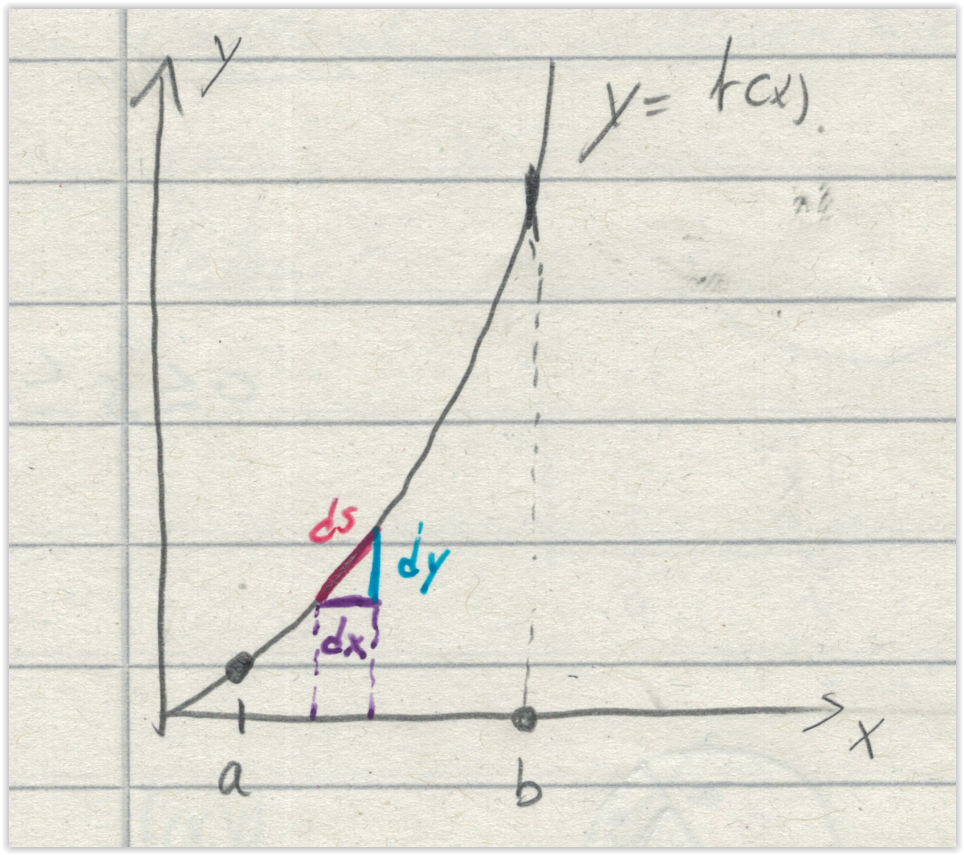
\includegraphics[width=0.4\linewidth]{kurvenlaenge.png}
			  \caption{Kurvenlänge}
			  \label{fig:lkurvenlaenge}
      \end{figure}
	  \end{bem}
	  
	  \subsubsection{Flächen geschlossener ebener Kurven}
	  \begin{equation}
	    F(c) = \frac{1}{2} \int\limits_a^b \big|\big(x(t)\dot{y}(t) - y(t)\dot{x}(t)\big)\big|dt
	  \end{equation}
  \subsection{Wegintegrale}
	  \subsubsection{Wegintegral erster Art}
	  \begin{definition}
	    Das Wegintegral erster Art ist definiert durch:
	    \begin{equation}
	      \int\limits_c \varrho \; dx = \int\limits_x \varrho \; ds = \int\limits_a^b \varrho(c(t)) \quad || \dot{c}(t)|| dt \label{eq:wegintegral_1}
	    \end{equation}
	  \end{definition}
	  \begin{bem}
	    Aus \eqref{fig:wegintegral_erster_2} geht
	    \begin{equation*}
	      ds = \sqrt{dx^2 + dy^2}
	    \end{equation*}
	    hervor. Damit folgt:
	    \begin{align*}
	      ds &= \sqrt{dx^2 + dy^2} = \frac{dt}{dt}  \sqrt{dx^2 + dy^2} = \frac{1}{dt} \sqrt{dx^2 + dy^2}dt \\
	      &=  \sqrt{\frac{1}{dt^2}(dx^2 + dy^2)} =  \sqrt{\left(\frac{dx}{dt}\right)^2 + \left(\frac{dy}{dt}\right)^2}
	    \end{align*}
	    Überträgt man das bekannte Integral aus dem $\R^2$, das mit $\int\limits_a^b f(x) dx$ gegeben ist, und  obigen Zusammenhang ein, so erhält man:
	    \begin{align*}
	      \int\limits_{t=a}^{t=b} f(x,y) ds = \int\limits_{t=a}^{t=b} f(x,y) \sqrt{dx^2 + dy^2}\\
	      = \int\limits_{t=a}^{t=b} \underbrace{f(x(t),y(t))}_{\text{Höhe}} \underbrace{\sqrt{\left(\frac{dx}{dt}\right)^2 + \left(\frac{dy}{dt}\right))^2} dt}_{ds}
	    \end{align*}
	  \end{bem}
	  \begin{figure}[H] 
		\centering
		\begin{minipage}{.5\textwidth}
		  \centering
		  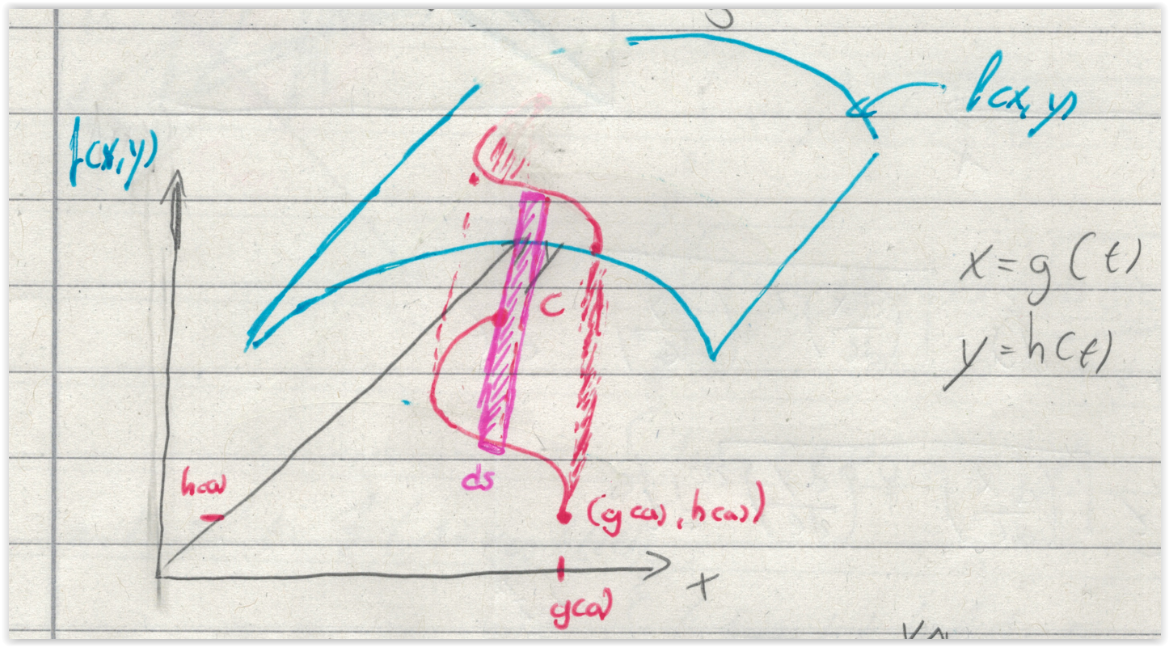
\includegraphics[width=0.9\linewidth]{wegintegral_erster_1.png}
		  \caption{Graphische Interpretation}
		  \label{fig:wegintegral_erster_1}
		\end{minipage}%
		\begin{minipage}{.5\textwidth}
		  \centering
		  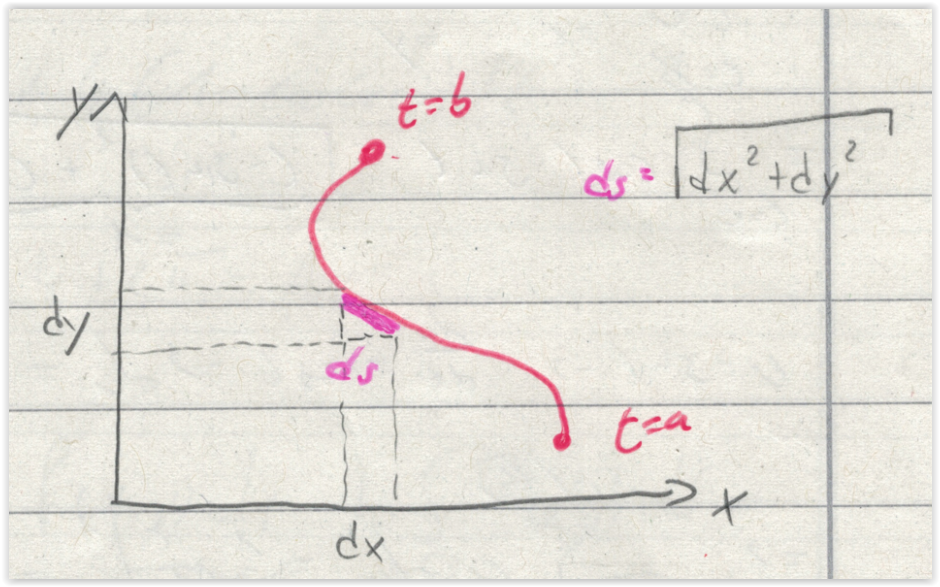
\includegraphics[width=0.8\linewidth]{wegintegral_erster_2.png}
		  \caption{Interpretation von \protect\eqref{eq:wegintegral_1}}
		  \label{fig:wegintegral_erster_2}
		\end{minipage}
		\end{figure}
		\begin{bem}
			\begin{itemize}
			  \item[a) ] Integrale sind unabhängig von der gewählten Parametrisierung.
			  \item[b) ] Falls $c$ geschlossen ist so schreibt man 
				  \begin{equation}
				    \oint\limits_c \varrho \; ds
				  \end{equation}
			\end{itemize}
		\end{bem}
		\subsubsection{Wegintegrale zweiter Art}
		\begin{definition}
		  Sei $f: D\rightarrow \R^d$ ein stetiges Vektorfreld mit $D\subset \R^d$ und sei $c:[a,b] \rightarrow D$ eine stückweise $C^1$-Kurve, dann heißt 
		  \begin{equation}
		    \int\limits_c <f(x), dx> = \int\limits_a^b <f\left(c(t)\right), \dot{c}(t)>dt
		  \end{equation}
		  das Wegintegral 2-ter Art. Falls $c$ geschlossen ist schreibt man
		  \begin{equation}
		    \oint\limits_c <f(x), dx>
		  \end{equation}
		\end{definition}
		\begin{bem}
		  Das Wegintegral ist unabhängig von der gewählten Parametrisierung.
		\end{bem}
		\begin{bem}
		  Eine Alternative ältere Schreibweise ist
		  \begin{equation*}
		    \int\limits_c <f(X),dX>
		  \end{equation*}
		  Achtung, es handelt sich nur um eine Schreibweise. Nicht das Skalarprodukt aus $f(X)$ und $dX$ bilden!
		\end{bem}
		\begin{definition}
  		Ein stetiges Vektorfeld $f$ heißt wirbelfrei, falls die Kurvenintegrale längs aller stückweise stetig diffbaren Kurven verschwinden, d.h.
  		\begin{equation}
  		  \oint\limits_c <f(x), dx> = 0
  		\end{equation}
  		gilt.
		\end{definition}
		Als Konsequenz daraus folgt die Wegunabhängigkeit der Kurvenintegrale für den Fall das $f$ wirbelfrei ist. Das heißt, ist $f$ wirbelfrei, so gilt:
		\begin{equation}
		  \int\limits_{c_1} <f(x),dx> = \int\limits_{c_2} <f(x),dx>
		\end{equation}
		für beliebige Wege $c_1$ und $c_2$ mit gleichen Anfangs- und Endpunkten.
		\begin{definition}
		  Eine Teilmenge $D \subset \R^d$ heißt (weg)-zusammenhängend, falls je zwei Punkte $x,y \in D$ durch eine stückweise $C^1$-Kurve in $D$ verbunden werden können.
		  \begin{figure}[H] 
			  \centering
			  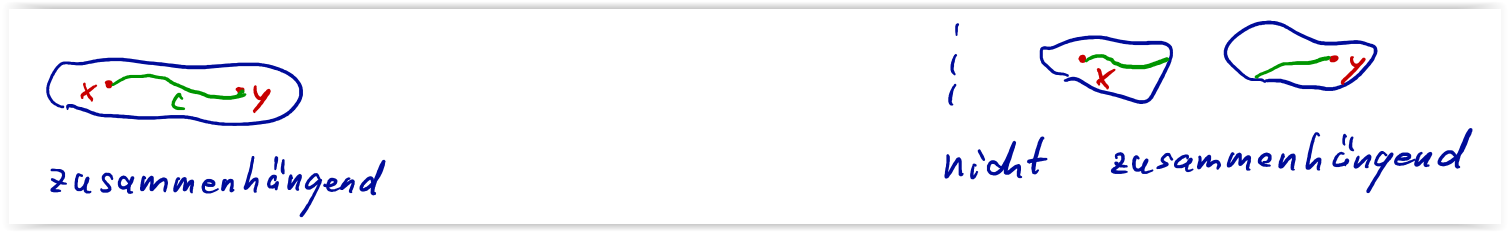
\includegraphics[width=0.8\linewidth]{zusammenhaengend.png}
			  \caption{Visualisierung zusammenhängend \protect\cite{HM12}}
			  \label{fig:zusammenhängend}
		  \end{figure}
		\end{definition}
		\subsubsection{Potential}
	  \begin{definition}
	    Sei $f:D\rightarrow \R^d$ ein Vektorfeld auf $D\subset \R^d$. Wir sagen $f$ ist ein gradientenfeld, falls es eine skalare $C^1$-Funktion $\varphi: D\rightarrow\R$ gibt, mit 
	    \begin{equation}
	    \nabla \varphi(x) = f(x)
	    \end{equation}
	    $\varphi$ heißt das Potential von $f$.
	  \end{definition}
    \begin{satz}
      Sei $D \subset \R^n$ offen und zusammenhängend und $f$ ein stetiges Vektorfeld auf $D$. 
      \begin{itemize}
        \item[a) ] Besitzt $f$ ein Potential $\varphi$, so gilt für alle stückweisen $C^1$-Kurven $c$, dass 
        \begin{equation}
          \int\limits_c <f(x),dx> = \varphi(c(b)) - \varphi(c(a))
        \end{equation}
        wobei $c:[a,b]\rightarrow \R^d$. D.h. das Wegintegral ist damit wegunabhängig und $f$ wirbelfrei.
        \item[b) ] Ist $f$ wirbelfrei, so besitzt $f$ ein Potential $\varphi$ mit der Darstellung 
        \begin{equation}
          \varphi(x) = \int\limits_{c_x} f(\tilde{x}),d\tilde{x}>
        \end{equation}
        wobei $c_x$ ein Weg nach $x$ mit fest gewähltem Startpunkt $x^*$ sein soll.
      \end{itemize}
    \end{satz}	  
	  \subsubsubsection{Berechnung von Potentialen}
	  Die notwendige (aber nicht hinreichende) Bedingung für die Existenz eines Potentials ist:
	  \begin{equation}
	    rot(\nabla \varphi) = 0 \Rightarrow rot(f) = 0 \Rightarrow Potential\;ex.  
	  \end{equation}
	  \begin{definition}
	    Ein Gebiet $G$ heißt einfach zusammenhängend, falls jeder geschlossene Weg in $G$ auf einen Punkt im Gebiet zusammen gezogen werden kann.
	    \begin{figure}[H] 
			  \centering
			  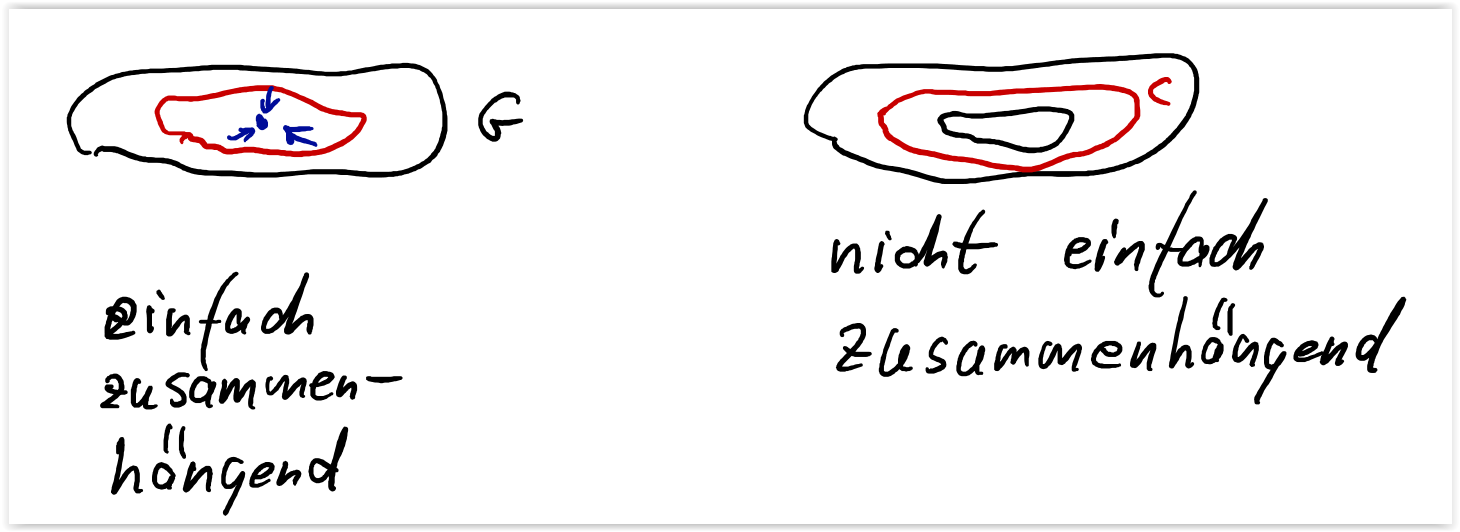
\includegraphics[width=0.8\linewidth]{einfach_zusammenhaengend.png}
			  \caption{Visualisierung einfach zusammenhängend \protect\cite{HM12}}
			  \label{fig:einfach_zusammenhängend}
		  \end{figure}
	  \end{definition}
	  
  \newpage
\bibliography{lit}

\end{document}